% !TEX root = perelman-geometry.tex
%!TEX TS-program = pdflatex
%!TEX encoding = UTF-8 Unicode



\setchapterpreamble[o]{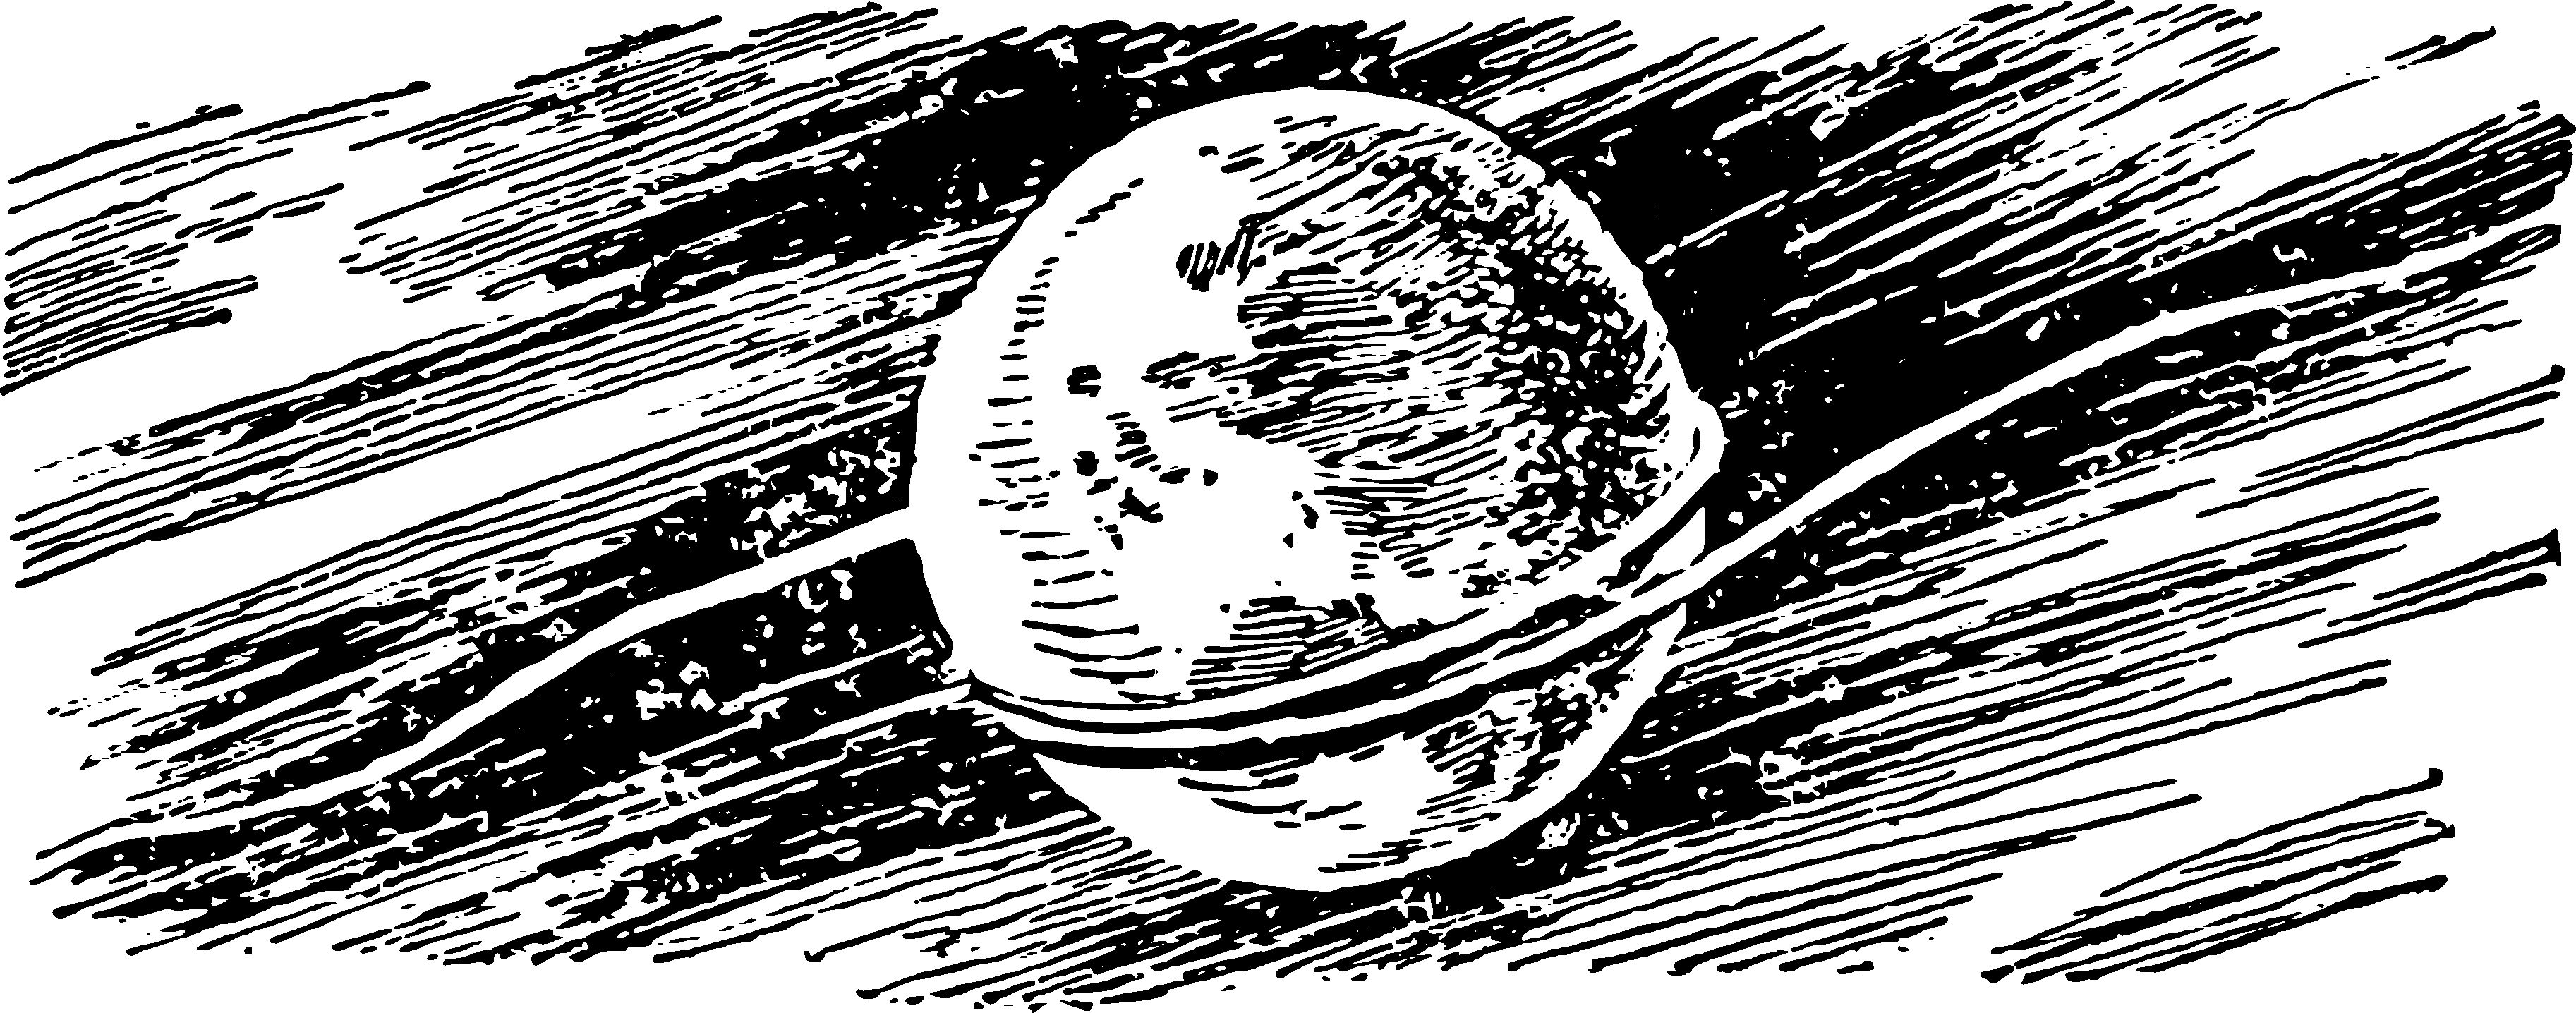
\includegraphics[width=1.2\textwidth]{figures/ch-09/fig-ch-09-head.pdf}\bigskip}

\chapter{Old And New About The Circle}
\label{ch-09}



\section{Practical Geometry of the Egyptians and Romans}
\label{sec-9.1}

Any schoolchild can now calculate the circumference based on its diameter much more accurately than the wisest priest of the ancient land of pyramids or the most skilled architect of great Rome. The ancient Egyptians believed that the circumference was 3.16 times longer than the diameter, while the Romans believed it was 3.12 times longer. However, the correct ratio is 3.14159\dots{} Egyptian and Roman mathematicians established the ratio of the circumference to the diameter not through strict geometric calculation, as later mathematicians did, but simply through experience. But why did they make such errors? Couldn't they just stretch a piece of string around a circular object and then straighten the string to measure it?

Undoubtedly, they did just that, but it should not be assumed that such a method would necessarily yield good results. Imagine, for example, a vase with a round bottom with a diameter of \SI{100}{\milli\meter}. The circumference of the bottom should be \SI{314}{\milli\meter}. However, in practise, measuring with a string, you are unlikely to get this length: it is easy to make a mistake of one millimetre, and then $\pi$ will turn out to be equal to 3.13 or 3.15. And if you consider that the diameter of the vase cannot be measured perfectly accurately either, and that an error of \SI{1}{\milli\meter} is quite probable here too, then you will see that for $\pi$, quite wide limits are obtained between 
\begin{equation*}%
\frac{313}{101} \qand \frac{315}{99},
\end{equation*}
i.e., in decimal fractions, between 
\begin{equation*}%
3.09 \qand 3.18.
\end{equation*}
You see, by determining $\pi$ in this way, we can get a result that does not coincide with 3.14: once it's 3.1, another time 3.12, the third time 3.17, and so on. Among them, by chance, there may be 3.14, but in the eyes of the calculator, this number will not carry more weight than the others.

Such an empirical approach cannot provide a somewhat acceptable value for $\pi$. In this regard, it becomes more understandable why the ancient world did not know the correct ratio of the circumference to the diameter and why it took the genius of Archimedes to find the value of $3\,\nicefrac{1}{7}$ for $\pi$ without measuring, relying solely on reasoning.



\section{``I know this and I remember it perfectly.''}
\label{sec-9.2}

In the \emph{Algebra} of the ancient Arab mathematician Mohammed ibn-Musa, we read the following lines about calculating the circumference:
\begin{quote}
The best way is to multiply the diameter by $3\,\nicefrac{1}{7}$. This is the fastest and easiest way. God knows the best. 
\end{quote}
Now we also know that Archimedes' number $3\,\nicefrac{1}{7}$ does not perfectly express the ratio of the circumference to the diameter. It has been theoretically proven that this ratio cannot be expressed as any exact fraction. We can only write it with some approximation, which, however, far exceeds the accuracy required for the strictest demands of practical life. The mathematician Ludolph in the 16th century, in Leiden, had the patience to calculate $\pi$ with 35 decimal places and bequeathed to have this value for $\pi$ carved on his tombstone\sidenote{At that time, the notation $\pi$ was not yet in use: it was introduced only from the middle of the 18th century by the famous Russian academician and mathematician Leonard Pavlovich Euler.}! (see \figr{fig-123}).

\begin{figure}[h!]
\centering
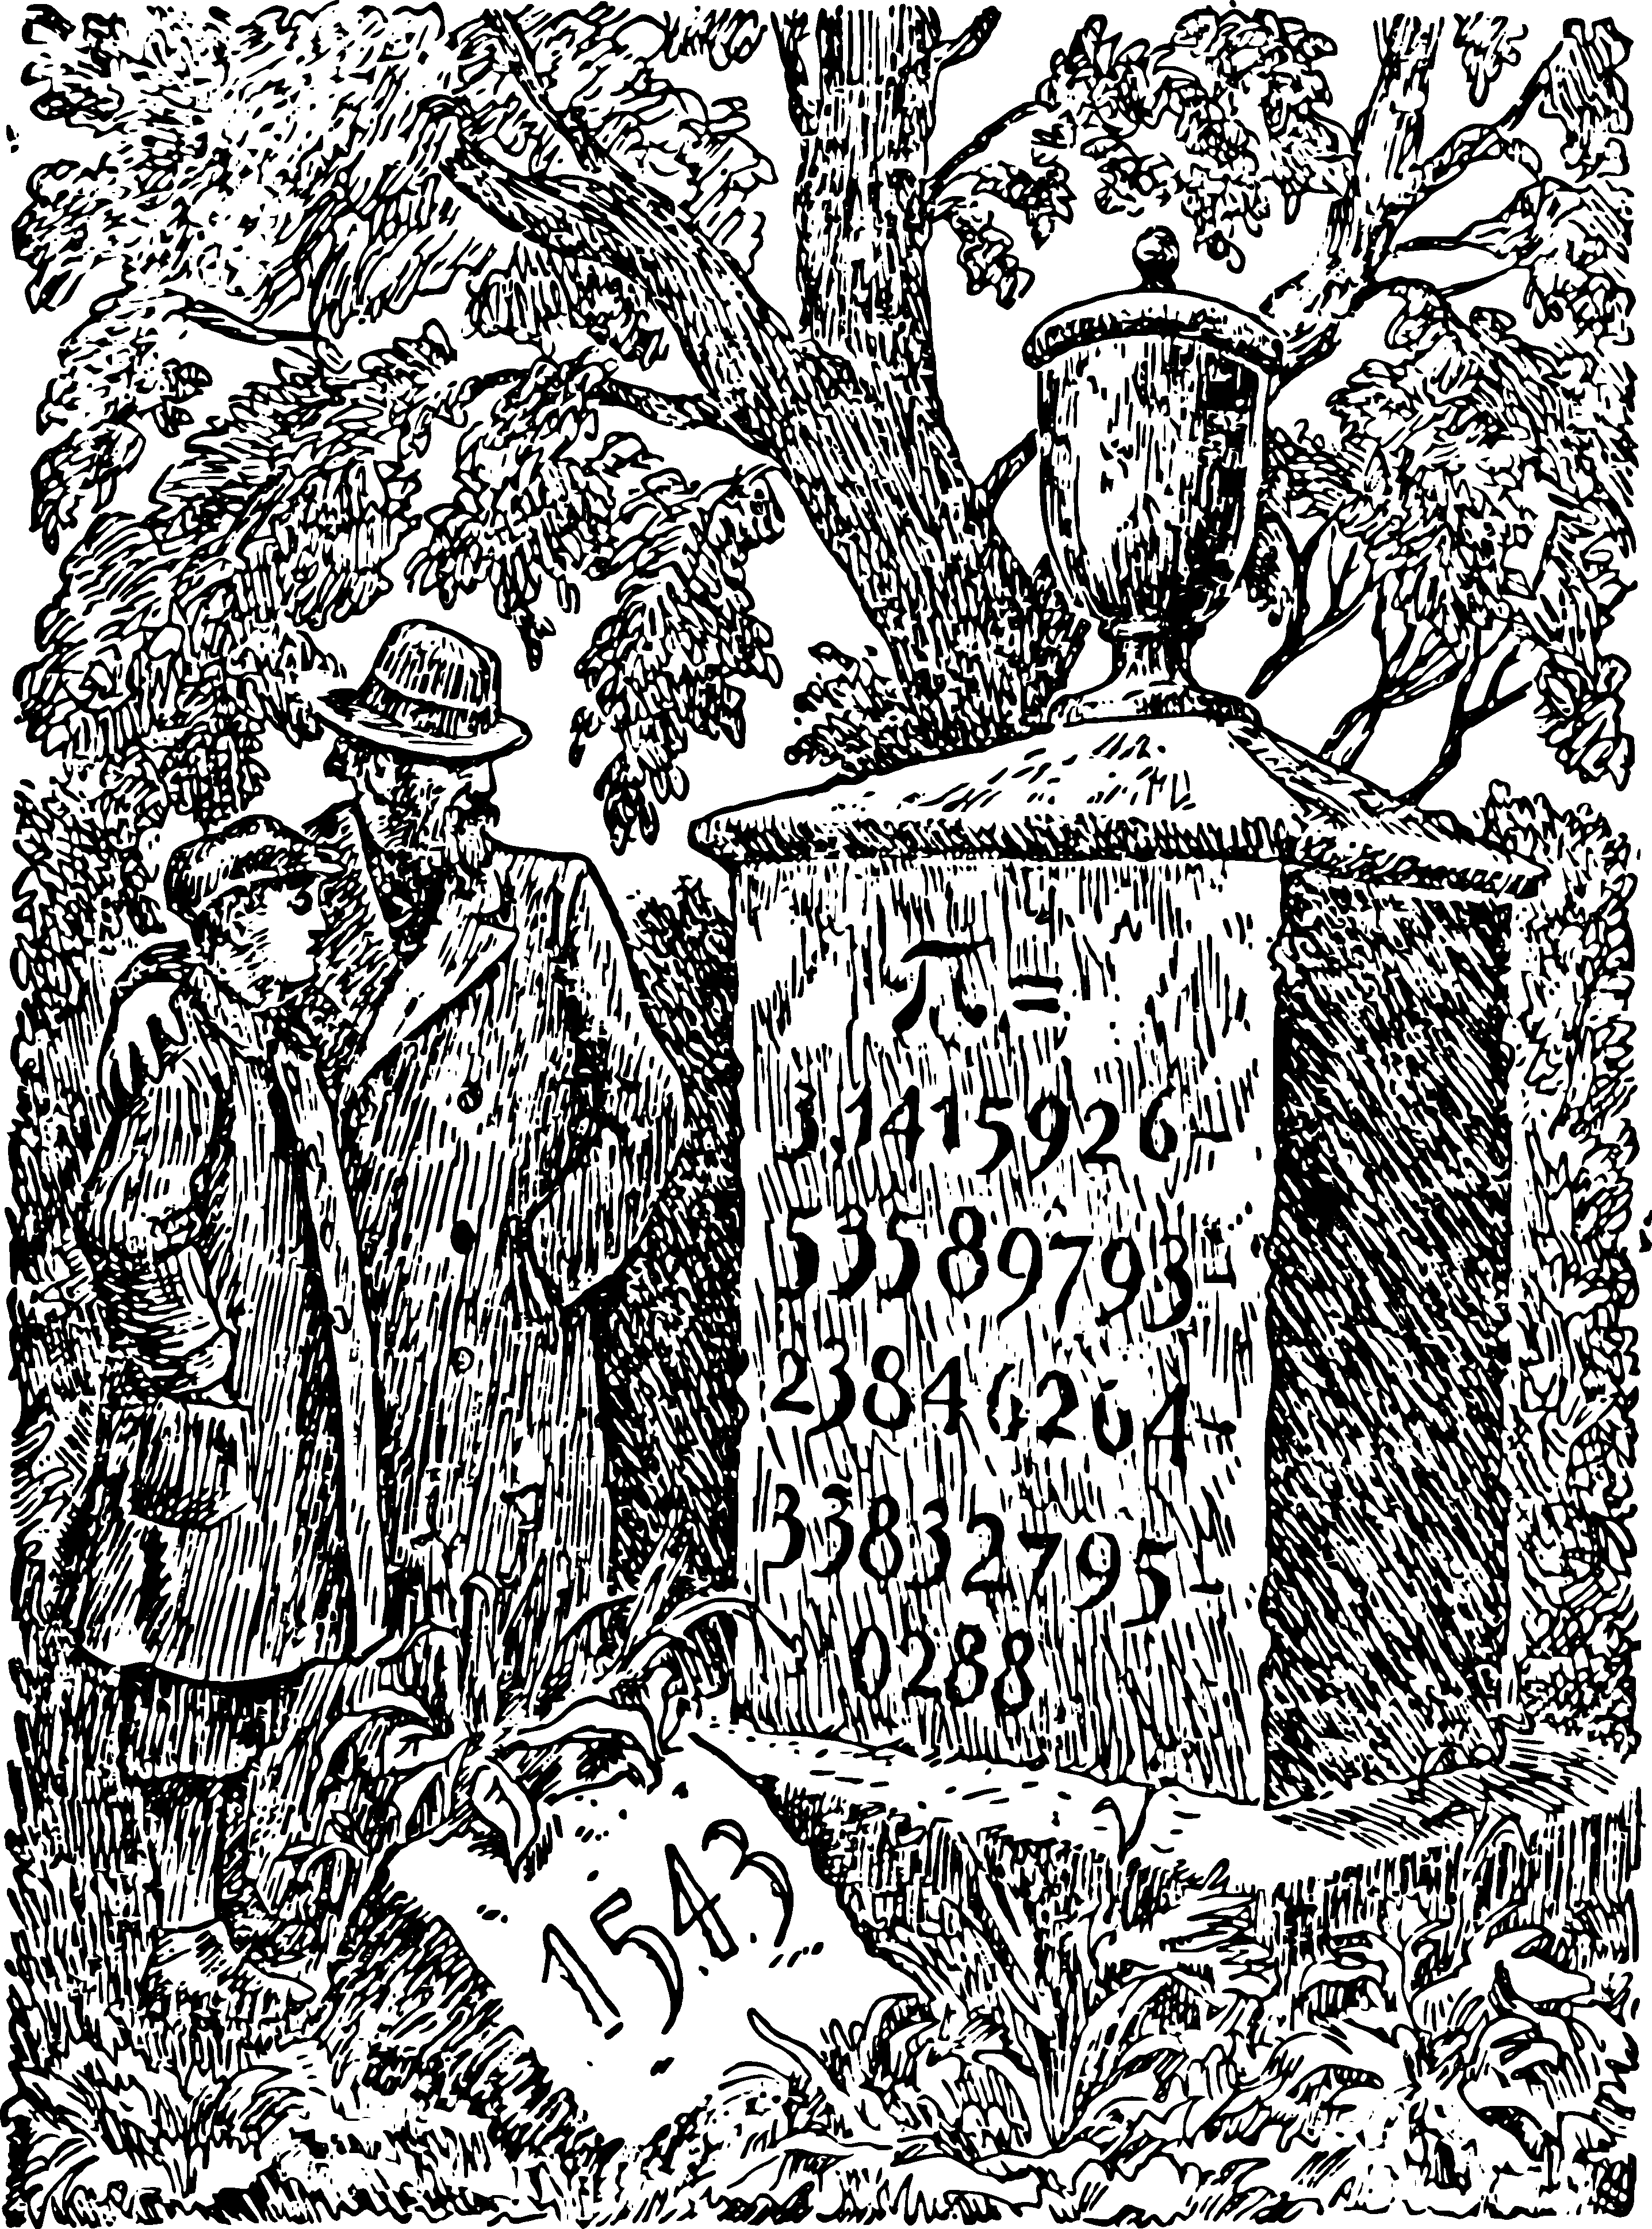
\includegraphics[width=0.7\textwidth]{figures/ch-09/fig-123.pdf}
\sidecaption{Mathematical epitaph.\label{fig-123}}
\end{figure}


Here it is: 
\begin{equation*}%
\num{3.14159265358979323846264338327950288}\dots{}
\end{equation*}
A certain Shanks in 1873 published a value of $\pi$ in which there were 707 decimal places after the comma! Such long numbers approximately expressing the value of $\pi$ have neither practical nor theoretical value. Only out of idleness and in pursuit of inflated ``records'' could there arise in our time a desire to "outdo" Shanks: in 1946-1947, Ferguson (Manchester City) and, independently of him, Weaver (from Washington) calculated 808 decimal places for the number $\pi$ and were pleased to find errors in Shanks's calculations starting from the 528th digit.\sidenote[][-2cm]{As of 2024, the value of $\pi$ has been calculated to 62,831,853,071,796 digits, that is \textbf{62 trillion} digits! For several different and modern methods to find value of $\pi$, please see the Wikipedia page \url{https://en.wikipedia.org/wiki/Pi}. -- \textsc{dm}}

If, for example, we wished to calculate the length of the Earth's equator with an accuracy of \SI{1}{\centi\meter}, assuming that we know the length of its diameter precisely, it would be sufficient for us to take only 9 digits after the decimal point in the number $\pi$. And by taking twice as many digits (18), we could calculate the circumference with a precision of not more than \SI{0.0001}{\milli\meter} (100 times smaller than the thickness of a hair!) for a circle with a radius equal to the distance from the Earth to the Sun.

Our compatriot, the mathematician Grave, vividly demonstrated the absolute uselessness of even the first hundred decimal places of $\pi$. He calculated that if we imagine a sphere with a radius equal to the distance from the Earth to Sirius, i.e., a number of kilometres equal to 132 followed by ten zeros: \num{132d10}, and fill this sphere with microbes, placing one billion (\num{d10}) microbes in each cubic millimetre of the sphere, and then arrange all these microbes in a straight line so that the distance between each pair of adjacent microbes again equals the distance from Sirius to Earth, then, taking this fantastic segment as the diameter of a circle, it would be possible to calculate the length of the resulting gigantic circumference with microscopic precision — up to \SI{0.000001}{\milli\metre}, by using 100 digits after the decimal point in the number $\pi$. French astronomer Arago correctly observes in this regard that ``in terms of accuracy, we would gain nothing if there were a relationship between the circumference and the diameter expressed by a number with complete accuracy.''

For ordinary calculations involving $\pi$, it is sufficient to remember two digits after the decimal point (3.14), and for more precise calculations, four digits (3.1416: we take the last digit as 6 instead of 5 because the following digit is greater than 5).

Small poems or vivid phrases are better retained in memory than numbers, so special poems or individual phrases are invented to memorise some numerical value of $\pi$. In works of this kind of mathematical poetry, words are chosen so that the number of letters in each word sequentially coincides with the corresponding digit of the number $\pi$.

There is a famous poem in English -- in 13 words, hence providing 12 digits after the decimal point in the number $\pi$; in German -- in 24 words, and in French, in 30 words! (and there are even ones in 126 words).

They are curious but too large, cumbersome. Among the students, E. Y. Terskov, a mathematics teacher at one of the secondary schools in the Moscow region, enjoys popularity for inventing the following stanza:

%\begin{quote}
\begin{small}
\gl{«Это я знаю и помню прекрасно».}
{3 1 4 1 5 9}
\end{small}

(`I know this and remember it perfectly.')\sidenote[][-2cm]{This sentence and the next ones in Russian are not really translatable with the number of characters in the words intact and corresponding to the numbers in $\pi$. I am giving the translations in English which do not match. I am also adding some alternative mnemonics in English. -- \textsc{dm}}
%\end{quote}

% See the discussion at https://tex.stackexchange.com/questions/717912/how-to-align-numbers-to-words-of-a-sentence-in-the-next-line/

And one of his students, Elya Cherikover, with the resourcefulness typical of our schoolchildren, composed a witty, slightly ironic continuation:

%\begin{quote}
\begin{small}
\gl{«Пи многие знаки мне лишни, напрасны»,}{2 6 5 3 5 8}\\
(`Pi, many digits are unnecessary for me, in vain,') 
%\end{quote}
\end{small}

In total, a twelve-word couplet is obtained:

\begin{small}
\gl{«Это я знаю и помню прекрасно, Пи многие знаки мне лишни, напрасны».}{3 1 4 1 5 9 2 6 5 3 5 8}
\end{small}

(`I know this and remember it perfectly, Pi, many digits are unnecessary for me, in vain.')

The author of this book, not daring to invent a poem, in turn suggests a simple and also quite sufficient prose phrase:

\begin{small}
\gl{«Что я знаю о кругах?»}{3 1 4 1 6}
\end{small}

(`What do I know about circles?') -- a question, secretly containing the answer.

Some English mnemonics:

\begin{small}
\gl{See I have a rhyme assisting, My feeble brain, its tasks ofttimes resisting.}{3 1 4 1 5 9 2 6 5 3 5 8 9}

\gl{Wow! I made a great discovery!}{3 1 4 1 5 9}

\gl{Can I have a small container of coffee?}{3 1 4 1 5 9 2 6}

\gl{How I want a drink, alcoholic of course, after the heavy lectures involving quantum mechanics.}{3 1 4 1 5 9 2 6 5 3 5 8 9 7 9}
\end{small}

A German menmonic (24 digits) \num{3 1 4 1 5 9 2 6 5 3 5 8 9 7 9 3 2 3 7 4 6 2 6 4}:

\begin{small}
\gl{Wie o dies $\pi$, Macht ernstlich, so vielen viele Müh’! Lernt immerhin, Jünglinge, leichte Verselein, Wie so zum Beispiel dies dürfte zu merken sein.}{3 1 4 1 5 9 2 6 5 3 5 8 9 7 9 3 2 3 7 4 6 2 6 4}
\end{small}

A French mnemonic (30 digits) \num{3 1 4 1 5 9 2 6 5 3 5 8 9 7 9 3 2 3 7 4 6 2 6 4 3 3 8 3 2 7 9}:

\begin{small}
\gl{Que j’aime à faire apprendre un nombre utile aux sages! Jmmortel Archimède, sublime ingénieur, Qui de ton jugement peut sonder la valeur? Pour moi ton problème eut de pareils avantages.}{3 1 4 1 5 9 2 6 5 3 5 8 9 7 9 3 2 3 7 4 6 2 6 4 3 3 8 3 2 7 9}
\end{small}

\clearpage
\section{Jack London's Error}
\label{sec-9.3}

The next passage from Jack London's novel \emph{The Little Lady of the Big House} provides material for geometric calculation:
\begin{quote}
In the middle of the field stood a steel pole, driven deep into the ground. From the top of the pole to the edge of the field stretched a cable, attached to a tractor. The mechanics pressed a lever -- and the engine started.

The machine moved forward on its own, describing a circle around the pole, which served as its center.

``To truly perfect the machine,'' Graham said, ``you need to turn the circle it describes into a square.''

``Yes, on a square field, this system wastes a lot of land.''

Graham made some calculations, then remarked:

``We lose approximately three acres out of every ten.''

``No less.''
\end{quote}

Readers are invited to verify this calculation.

\ans The calculation is incorrect: less than 0.3 of the total land is lost. Let's assume that the side of the square is $a$. The area of such a square is $a^{2}$. The diameter of the inscribed circle is also $a$, and its area is $\pi a^{2}/4$. The lost part of the square plot is
\begin{equation*}%
a^{2} - \frac{\pi a^2}{4} = \left(1 - \frac{\pi}{4} \right) a^{2}= 0.22 \, a^{2}.
\end{equation*}
We can see that the unused part of the square field amounts not to 30\% as the characters in the American novelist's story believed, but only about 22\%.


\section{Dropping a Needle}
\label{sec-9.4}


The most original and unexpected method for approximating the number $\pi$ is as follows. Take a short (about two centimeters) sewing needle -- preferably with a blunted tip to ensure uniform thickness -- and draw a series of thin parallel lines on a sheet of paper, with each line spaced apart by twice the length of the needle.

\begin{figure}[h!]
\centering
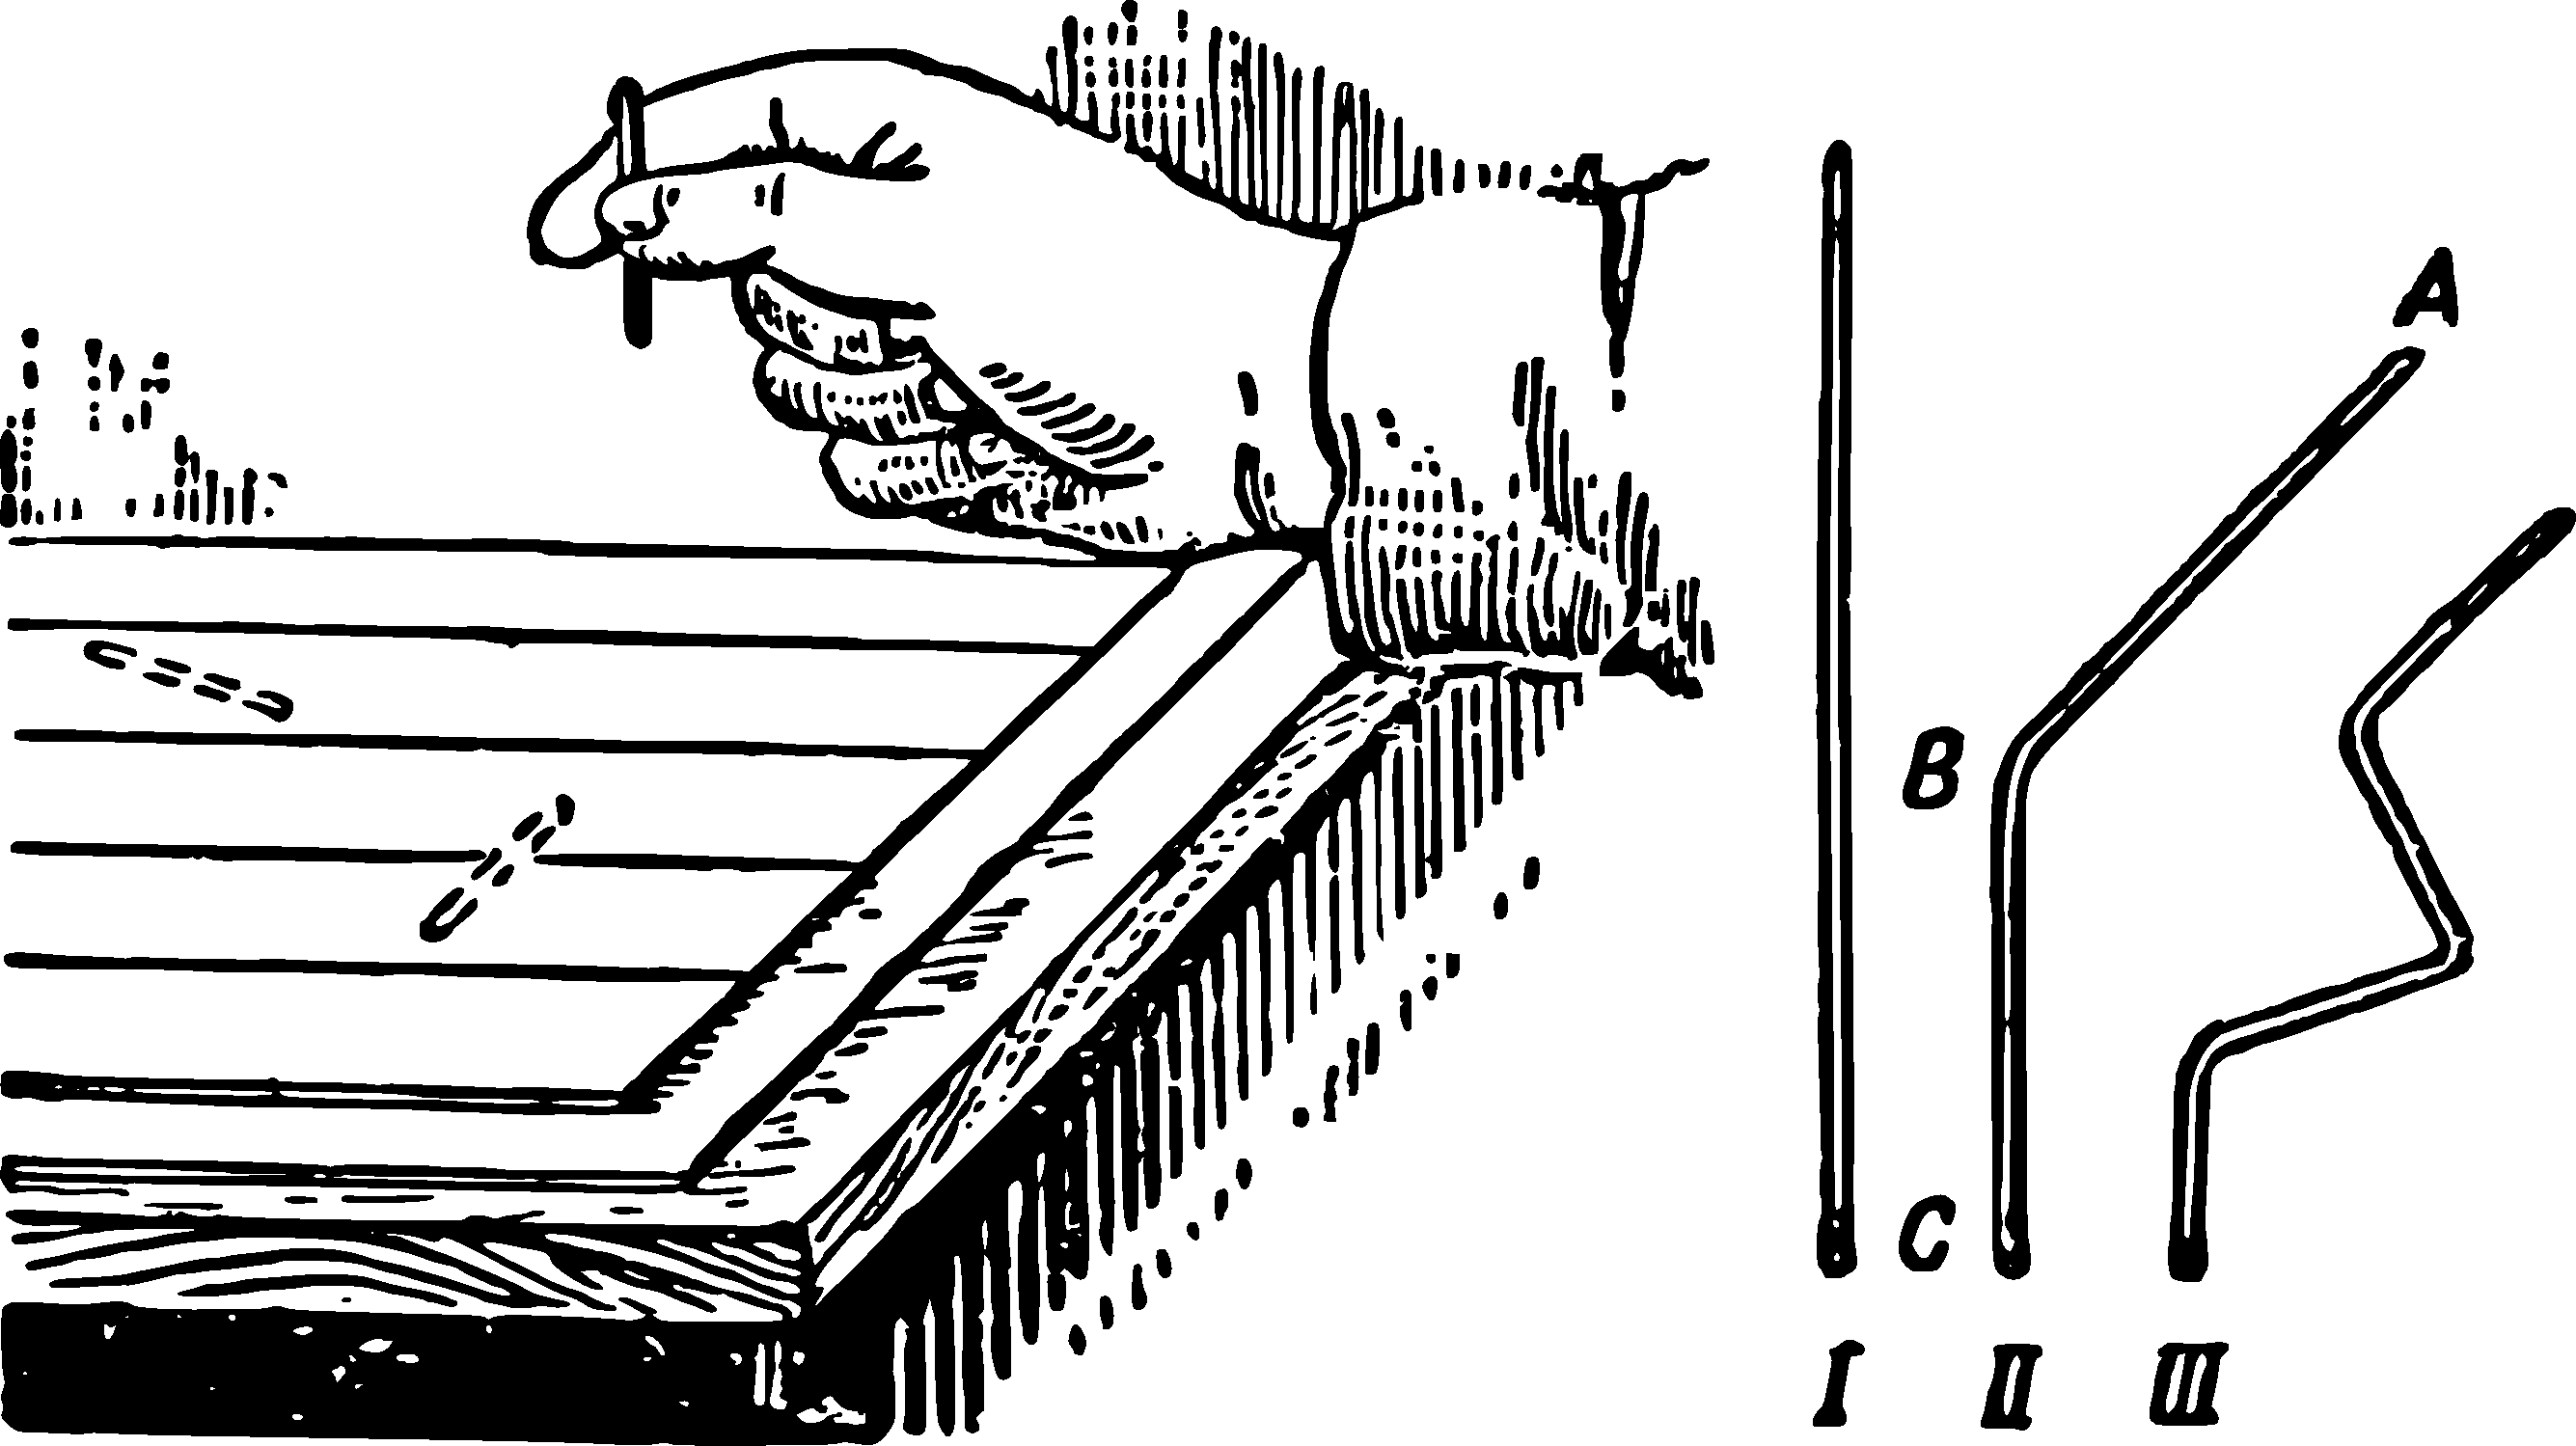
\includegraphics[width=0.9\textwidth]{figures/ch-09/fig-124.pdf}
\sidecaption{Buffon's needle-throwing experiment.\label{fig-124}}
\end{figure}

Then, drop the needle onto the paper from a certain (arbitrary) height and observe whether the needle crosses one of the lines or not (see \figr{fig-124}, left). To prevent the needle from bouncing, place a piece of thin paper or cloth under the paper sheet. Repeat the dropping of the needle many times, for example a hundred or, even better, a thousand times, each time noting whether there was a crossing or not.\sidenote{The intersection should also be considered the case when the needle only rests against the end of the drawn line.} If you then divide the total number of needle drops by the number of instances where a crossing was observed, the result should approximate the value of $\pi$, more or less accurately.

Let's explain why this happens. Let the most likely number of needle crossings be denoted as  $K$, and the length of our needle be \SI{20}{\milli\meter}. In the case of a crossing, the point of intersection must, of course, lie on one of these millimeters, and no one millimeter, nor any part of the needle, has any advantage in this regard over the others. Therefore, the most likely number of crossings for each individual millimeter is $K/20$. For a segment of the needle of \SI{3}{\milli\meter}, it is $ 3K/20$, for a segment of \SI{11}{\milli\meter} -- $ 11K/20$, and so on. In other words, the most likely number of crossings is directly proportional to the length of the needle.

This proportionality is maintained even if the needle is bent. Let the needle be bent in the form shown in figure \figr{fig-124}, (\emph{II} right), with segment $AB = \SI{11}{\milli\meter}$ and $BC = \SI{9}{\milli\meter}$. For segment $AB$, the most likely number of crossings is $11K/20$, and for segment $BC$ it is $9K/20$. For the entire needle it is $ 11K/20 + 9K/20$, which still equals $K$. We can bend the needle in a more intricate way (\figr{fig-124}, (\emph{III} right)) -- this would not change the number of crossings. (Note that with a bent needle, crossings are possible with two or more parts of the needle at once; such crossings should be counted as 2, 8, etc., because the first is counted for one part of the needle, the second for another, and so on.)

Now imagine that we are dropping a needle, bent into the shape of a circle with a diameter equal to the distance between the lines (it is twice the length of our needle). Such a ring must intersect any line twice each time (or touch two lines once each -- in any case, two encounters occur). If the total number of drops is $N$, then the number of encounters is $2N$. Our straight needle is shorter than this ring by as many times as the radius is less than the circumference, which is $2\pi$ times. But we have already established that the most likely number of crossings is proportional to the length of the needle. Therefore, the most likely number $(K)$ of crossings of our needle should be less than $2M$ by $2\pi$ times, i.e., equal to $N/\pi$. Hence,
\begin{equation*}%
 \pi = \frac{\text{number of drops}}{\text{number of crossings}}.\end{equation*}

The more drops observed, the more accurate the expression for $\pi$ becomes. The Swiss astronomer R. Wolff in the middle of the last century observed 5000 needle drops on grid paper and obtained $\pi$ as 3.159\dots{} an expression, however, less precise than the Archimedean number.

As you can see, the ratio of the circumference to the diameter is determined here experimentally, and what is more curious -- neither a circle nor a diameter is drawn, meaning no compass is used. A person with no knowledge of geometry or even circles can determine $\pi$ using this method if they patiently perform a very large number of needle drops.

%\vspace{2cm}

\section{Straightening a Circle Problem}
\label{sec-9.5}

\begin{marginfigure}
\centering
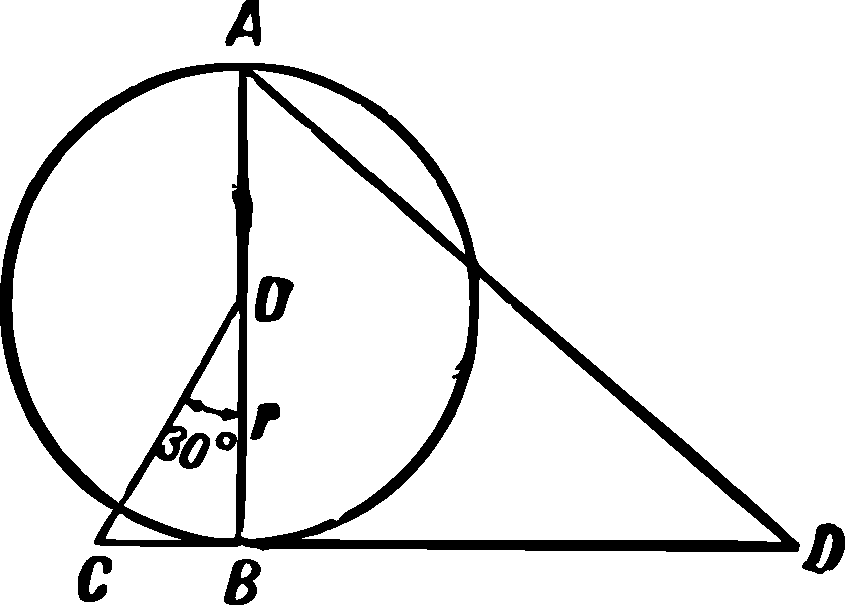
\includegraphics[width=\textwidth]{figures/ch-09/fig-125.pdf}
\sidecaption{An approximate geometric method of rectifying a circle.\label{fig-125}}
\end{marginfigure}

For many practical purposes, it is sufficient to take $\pi$ as 3 and  1/7 straighten the circle by laying out its diameter on any straight line 3 \, 1/7 times (dividing the segment into seven equal parts can be done quite accurately, as is well known). There are other approximate methods for straightening a circle used in practise by craftsmen such as carpenters, tinsmiths, and so on. We won't discuss them here, but we'll mention one fairly simple method of straightening that yields results with extremely high accuracy.



If it is necessary to straighten a circle $O$ with radius $r$ (see \figr{fig-125}), then draw the diameter $AB$, and at point $B$, draw line $CD$ perpendicular to it. From the centre $O$, draw line $OC$ at an \ang{30} angle to $AB$. Then, on line $CD$ from point $C$, mark off three radii of the given circle and connect the resulting point $D$ to $A$: the length of segment $AD$ equals the length of half the circumference. If segment $AD$ is doubled in length, an approximately straightened circle $O$ is obtained. The error is less than $0.0002\, r$.

On what basis is this construction founded?

\ans According to the Pythagorean theorem, 
\begin{equation*}%
CB^{2} + OB^{2} = OC^{2}.
\end{equation*}
Denoting the radius $OB$ as $r$ and considering that $CB = OC/2$ (as a leg, lying opposite an \ang{30} angle), we get: 
\begin{equation*}%
CB^{2} + r^{2} = 4CB^{2}, 
\end{equation*}
from which,
\begin{equation*}%
CB = \frac{r \sqrt{3}}{3}.
\end{equation*}
Next, in triangle $ABD$:
\begin{align*}%
BD & =  CD - CB = 3r - \frac{r\sqrt{3}}{3}.\\
AD & = \sqrt{BD^{2} + 4r^{2}} = \sqrt{\left( 3r - \frac{r \sqrt{3}}{3} \right)^{2} + 4r^{2}}, \\
& = \sqrt{9r^{2} - 2r^{2}\sqrt{3} + r^{2}/3 + 4r^{2}}, \\
& = 3.14153\, r.
\end{align*}
Comparing this result with one obtained with high precision for $\pi$ (approximately $( \pi = 3.14153)$, we see that the difference is only $0.00006\, r$. If we were to straighten a circle with a radius of 1 unit using this method, the error would be only 0.00006 meters for the semicircle, and for the full circle, it would be 0.00012 meters, or 0.12 millimetres (roughly three times the thickness of a hair).


\section{Squaring the Circle}
\label{sec-9.6}

It is unlikely that any reader has never heard of the ``squaring of the circle'' -- that most famous problem in geometry that mathematicians have been working on for twenty centuries. I am even confident that among the readers there are those who have tried to solve this problem themselves. However, even more readers may wonder what exactly the difficulty lies in resolving this classic unsolvable problem. Many, accustomed to repeating from others that the problem of squaring the circle is unsolvable, do not have a clear understanding of the essence of the problem or the difficulty of its resolution.

In mathematics, there are many problems much more interesting both theoretically and practically than the problem of squaring the circle. However, none has gained such popularity as this problem, which has long become a byword. For two millennia, outstanding professional mathematicians and countless crowds of amateurs have worked on it.

To square the circle" means to draw a square whose area is exactly equal to the area of a given circle. Practically, this problem arises very often, but precisely in practise, it can be solved with any degree of accuracy. The famous ancient problem, however, requires that the drawing be done perfectly using only two types of drawing operations: 
\begin{enumerate}
\item drawing a circle of a given radius around a given point; 
\item drawing a straight line through two given points.
\end{enumerate}
In short, it is necessary to make a drawing using only two drawing instruments: a compass and a straightedge.


In other words, it is necessary to make a drawing using only two drawing instruments: a compass and a straightedge.

Among non-mathematicians, there is a widespread belief that all the difficulty lies in the fact that the ratio of the circumference to its diameter (the famous number $\pi$) cannot be expressed by a finite number of digits. This is true only to the extent that the solvability of the problem depends on the peculiar nature of the number $\pi$. Indeed: transforming a rectangle into a square with equal area is an easily and precisely solvable problem. But the problem of squaring the circle is reduced to constructing -- with a compass and a straightedge -- a rectangle equal in area to the given circle. From the formula for the area of a circle, $S = \pi r^2$, or (which is the same thing) $S = \pi \times r \times r$, it is clear that the area of the circle is equal to the area of such a rectangle, where one side is $r$ and the other is $\pi$ times larger. As you know, $\pi$ is not exactly equal to 3 \, 1/7, or 3.14, or even 3.14159. The series of digits expressing this number goes to infinity.

The particularity of the number $\pi$, its irrationality\sidenote{The peculiarity of an irrational number is that it cannot be expressed as any exact fraction.}, was established by mathematicians Lambert and Legendre back in the 18th century. Yet, the knowledge of the irrationality of $\pi$ did not stop the efforts of those versed in mathematics, the ``quadraturists''. They understood that the irrationality of $\pi$ itself does not make the problem hopeless. There are irrational numbers that geometry can ``construct'' perfectly accurately. For example, suppose we need to draw a segment that is longer than a given one by $\sqrt{2}$ times. The number $\sqrt{2}$, like $\pi$, is irrational. Nevertheless, nothing could be easier than drawing the desired segment: let's remember that $\sqrt{2}$ is the side of a square inscribed in a circle with a radius of 1, because it amounts to constructing a regular 64-gon.



Every schoolchild also easily copes with constructing the segment $ a \sqrt{3}$ (the side of an equilateral inscribed triangle). Even constructing such a seemingly complex irrational expression presents no particular difficulty:
\begin{equation*}%
\sqrt{2 - \sqrt{2 + \sqrt{2 + \sqrt{2 +\sqrt{2}}}}}.
\end{equation*}
As we can see, an irrational multiplier, entering into the expression, does not always render this expression impossible to construct with a compass and straightedge. The unsolvability of squaring the circle is not entirely due to the fact that the number $\pi$ is irrational, but to another peculiarity of this same number. Namely, the number $\pi$ is not algebraic, i.e., it cannot be obtained as the solution to any equation with rational coefficients. Such numbers are called ``transcendental''.

A mathematician of the 19th century proved that the number $\pi$ is transcendental. This expression for $\pi$ would solve the problem of squaring the circle if the number of operations involved were finite (then the expression could be geometrically constructed). But since the number of square root extractions in this expression is infinite, Vieta's expression does not help the cause.

So, the unsolvability of the problem of squaring the circle is due to the transcendence of the number $\pi$, i.e., it cannot be the result of solving an equation with rational coefficients. This peculiarity of the number $\pi$ was rigorously prooven in 1889 by the German mathematician Lindemann. In essence, this scientist should be considered the only person who solved the squaring of the circle problem, despite the fact that his solution is negative -- it asserts that the desired construction is geometrically impossible. Thus, in 1889 the centuries-long efforts of mathematicians in this direction were concluded; however, unfortunately, the fruitless attempts of numerous amateurs, insufficiently familiar with the problem, have not ceased.

This is the state of affairs in theory. As for practise, it does not require an exact resolution of this famous problem at all. The belief of many that solving the problem of squaring the circle would have a huge significance for practical life is a profound misconception. For everyday needs, it is perfectly sufficient to have good approximate solutions to this problem.


Practically, the quest for squaring the circle became futile once the first 7-8 accurate digits of the number $\pi$ were found. For the needs of practical life, it is entirely sufficient to know that $\pi$ is approximately equal to 3.1415926. No measurement of length can provide a result expressed in more than seven significant digits. Therefore, having more than eight digits for $\pi$ is useless: it does not improve the precision of calculations\sidenote{See \emph{Entertaining Mathematics} by Yakov I. Perelman.}. Even if the radius is expressed with seven significant digits, the circumference will not contain more than seven reliable digits, even if $\pi$ is taken to a hundred digits. The fact that ancient mathematicians expended enormous effort to obtain possibly longer values of $\pi$ has no practical significance. Moreover, the scientific value of these works is negligible. It's simply a matter of patience. If you have the inclination and leisure, you can find up to 1000 digits for $\pi$ using, for example, the following infinite series discovered by Leibniz\sidenote{A lot of patience would be required for such a calculation because to obtain, for example, a six-digit $\pi$ , it would be necessary to take in the specified series not a few, not a little -- 2,000,000 terms.}:
\begin{equation*}%
\frac{\pi}{4} = 1 - \frac{1}{3} + \frac{1}{5} - \frac{1}{7} + \frac{1}{9} - \frac{1}{11} + \ldots{}
\end{equation*}
But this would be an unnecessary arithmetic exercise, far from contributing to the resolution of the famous geometric problem.

The French astronomer Arago, mentioned earlier, wrote the following about this:
\begin{quote}
The seekers of the squaring of the circle continue to engage in solving a problem whose impossibility is now positively proven and which, even if it could be achieved, would be of no practical interest. It is not worth dwelling on this subject: the mentally ill, striving for the discovery of the squaring of the circle, are not swayed by any arguments. This mental illness has existed since ancient times.
\end{quote}
And he ironically concludes:
\begin{quote}
The academies of all countries, fighting against the seekers of quadrature, have noticed that this disease usually intensifies in the spring.
\end{quote}

\section{Triangle of Bing}
\label{sec-9.7}

Let's consider one of the approximate solutions to the problem of squaring the circle, very convenient for practical purposes.

\begin{marginfigure}
\centering
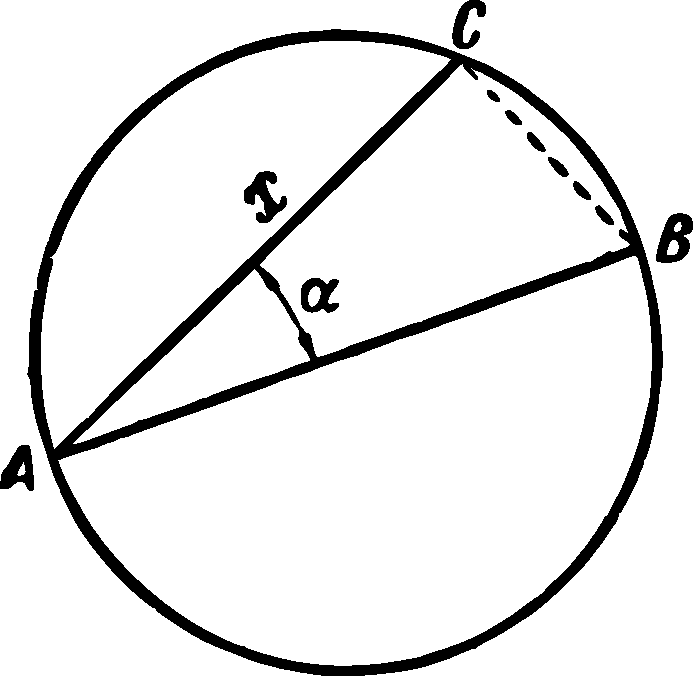
\includegraphics[width=\textwidth]{figures/ch-09/fig-126.pdf}
\sidecaption{The method of the Russian engineer Bing (1836).\label{fig-126}}
\end{marginfigure}


The method consists of computing (see \figr{fig-126}) the angle $\alpha$, under which it is necessary to draw, to the diameter $AB$, the chord $AC = x$, which is one side of the desired square. To find the value of this angle, one will have to resort to trigonometry:
\begin{equation*}%
\cos \alpha = \frac{AC}{AB} = \frac{x}{2r},
\end{equation*}
where $r$ is the radius of the circle.

This means that the side of the desired square $x = 2r \cos \alpha$, and its area is equal to $4r^{2} cos^{2} \alpha$. On the other hand, the area of the square is equal to the area of the given circle $\pi r^{2}$.

Thus,
\begin{align*}%
4r^{2} \cos^{2} \alpha & = \pi r^{2}, \,\, \text{from which,}\\
cos^{2} \alpha & = \frac{\pi}{4}, \,\, \text{and,} \\
cos \alpha & = \frac{1}{2} \sqrt{\pi} = 0.886.
\end{align*}
By looking up in the tables, we find:
\begin{equation*}%
\alpha = \ang{27;36}.
\end{equation*}
So, by drawing in this circle a chord at an angle of \ang{27;36} to the diameter, we immediately obtain the side of the square whose area is equal to the area of the given circle. Practically, one prepares a drawing triangle\sidenote{This convenient method was proposed in 1886 by the Russian engineer Bing; the mentioned drawing triangle is named after its inventor as the `Triangle of Bing.'}, one of the acute angles of which is \ang{27;36} (and the other is \ang{62;24}). Having such a triangle, one can immediately find the side of a square equal to it for each given circle.

For those who want to make such a drawing triangle for themselves, the following instruction may be useful.

Since the tangent of the angle \ang{27;36} is 0.5923, or $\approx 23/44$, then the legs of such a triangle are related as 23:44. Therefore, by making a triangle with one leg, for example, \SI{22}{\centi\meter}, and the other \SI{11.5}{\centi\meter}, we will have what is required. It goes without saying that such a triangle can be used as an ordinary drawing instrument.


\section{Head or Feet}
\label{sec-9.8}

It seems that one of Jules Verne's characters calculated which part of his body travelled the longest distance during his circumnavigation -- his head or the tips of his feet. This is a very instructive geometric problem if framed in a certain way. We'll present it as follows:


\ques Imagine that you've travelled around the Earth along the equator. By how much has the top of your head travelled a greater distance than the tip of your feet?


\ans The feet have travelled a distance of $2\pi R$, where $R$ is the radius of the Earth. Meanwhile, the top of the head has travelled a distance of $2\pi(R + 1.7)$, where 1.7 meters is the height of a person. The difference in distances is $2\pi(R + 1.7) - 2\pi R = 2\pi(1.7) = \SI{10.7}{\meter}$. Thus, the head has travelled 10.7 meters more than the feet.

Interestingly, the final answer does not involve the radius of the Earth. Therefore, the result would be the same on Earth, Jupiter, or even the smallest planetoid. In general, the difference in lengths between two concentric circles depends only on the distance between them, not their radii. Adding one centimetre to the radius of the Earth's orbit would increase its length by the same amount as an equal increase in the radius of any other circle.

This geometric paradox\sidenote{A paradox is a truth that seems implausible, in contrast to sophism -- a false position that has the appearance of being true.} underlies the following interesting problem, found in many collections of geometric puzzles.

If a wire is stretched around the Earth's equator and its length is increased by 1 meter, would a mouse be able to pass between the wire and the Earth?

The usual answer is that the gap would be thinner than a hair: what is one meter compared to 40 million meters of the Earth's equator! However, the actual size of the gap is:
\begin{equation*}%
\frac{100}{2 \pi} \si{\centi\meter} = \SI{16}{\centi\meter}.
\end{equation*}
Not only a mouse, but even a large cat could pass through such a gap.


\section{Wire Along the Equator Problem}
\label{sec-9.9}


\ques Now, imagine that the Earth is tightly encased along the equator with a steel wire. What would happen if this wire cooled by \SI{1}{\degreeCelsius}? As the wire cools, it should shorten. If it doesn't break or stretch, how deeply will it embed into the soil?



\ans At first glance, such a slight decrease in temperature, just by \SI{1}{\degreeCelsius}, might not seem to cause a noticeable embedding of the wire into the ground. However, calculations show otherwise.

Cooling by \SI{1}{\degreeCelsius}, the steel wire shortens by one hundred thousandth of its length. With a length of 40 million meters (the length of the Earth's equator), the wire should shorten, as easily calculated, by 400 meters. However, the radius of this circle made by the wire will decrease not by 400 meters, but much less. To determine how much the radius will decrease, we need to divide 400 meters by 6.28, i.e., by $2\pi$.

The result is about \SI{64}{\meter}. Therefore, the wire, cooling by just \SI{1}{\degreeCelsius} under the given conditions, would embed into the ground not just by a few millimeters, as one might think, but by more than \SI{60}{\meter}!


\section{Facts and Calculations}
\label{sec-9.10}


\ques You have eight equal circles in front of you (see \figr{fig-127}). Seven of them are shaded -- immovable, while the eighth (light one) rolls over them without slipping. How many revolutions will it make after going around the immovable circles once?

\begin{figure}[h!]
\centering
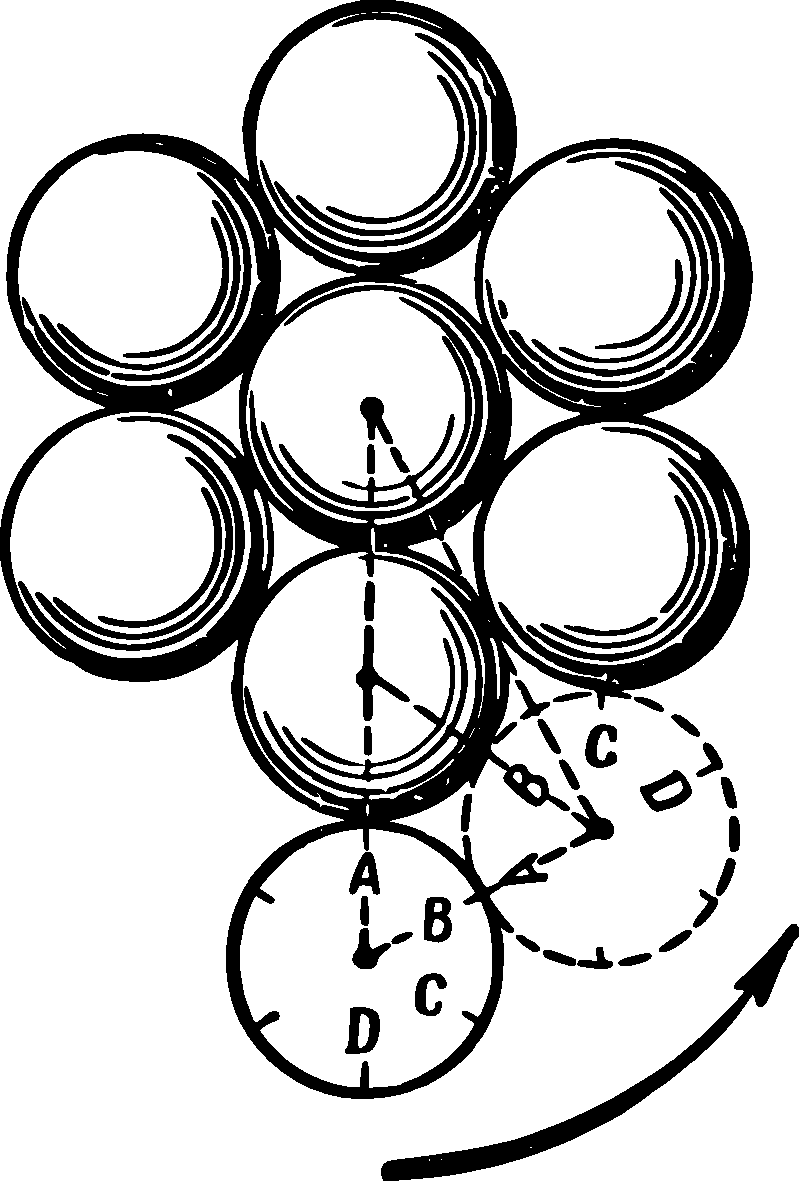
\includegraphics[width=0.55\textwidth]{figures/ch-09/fig-127.pdf}
\sidecaption{How many turns will the light circle make, bypassing the fixed shaded circles?\label{fig-127}}
\end{figure}


You can certainly figure this out practically: place eight coins of equal value on the table, for example, eight coins, arrange them as shown in the picture, and, pressing down on seven coins, roll the eighth one over them. To determine the number of revolutions, for example, watch the position of the number written on the coin. Every time the number returns to its initial position, the coin will have completed one full revolution around its centre.

Perform this experiment not just in your imagination but in reality, and you will find that the coin makes a total of four revolutions.

Now let's try to arrive at the same answer through reasoning and calculations. Let's find out, for example, how much arc each immovable circle covers as the rolling circle moves. To do this, imagine the movement of the rolling circle from the ``hill'' $A$ to the nearest ``valley'' between two immovable circles (shown by the dashed line in \figr{fig-127}).

From the diagram, it is easy to determine that the arc $AB$, along which the circle rolled, measures \ang{60}. On the circumference of each immovable circle, there are two such arcs; together, they make up an arc of \ang{120} or $\nicefrac{1}{3}$ of the circumference.

Therefore, the rolling circle completes $\nicefrac{1}{3}$ of a revolution, covering $\nicefrac{1}{3}$ of each immovable circle. There are a total of six immovable circles; thus, the rolling circle will complete $\nicefrac{1}{3} \times 6 = 2$ revolutions.

This results in a discrepancy with the observations! But `facts are stubborn things.' If observation does not confirm the calculation, then there must be a defect in the calculation.

Find the defect in the reasoning provided.

\ans  The point is that when the circle rolls without slipping along a straight segment equal to $\nicefrac{1}{3}$ of its circumference, it indeed completes $\nicefrac{1}{3}$ of a revolution around its centre. This statement becomes untrue, not reflecting reality, when the circle rolls along an arc of a curved line. In the problem under consideration, as the rolling circle traverses an arc, for example, one-third of the length of its circumference, it completes not $\nicefrac{1}{3}$ but $\nicefrac{2}{3}$ of a revolution. Therefore, passing through six such arcs, it completes
\begin{equation*}
6 \times \frac{2}{3} = 4\,\,\text{revolutions!}
\end{equation*}
You can visually confirm this. The dashed line in \figr{fig-127} depicts the position of the rolling circle after it has rolled along the arc $AB\,\, (=\ang{60})$ of an immovable circle, i.e., along an arc constituting 1/6 of the circumference. In the new position, the highest point on its circumference is occupied not by point $A$ but by point $C$, which, as you can see, corresponds to a rotation of the points on the circumference by \ang{120}, i.e., by $\nicefrac{1}{3}$ of a full revolution. A ``path'' of \ang{120} corresponds to $\nicefrac{2}{3}$ of a full revolution of the rolling circle.

So, if the circle rolls along a curved (or piecewise linear) path, it completes a different number of revolutions than when it rolls along a straight path of the same length.

Let's dwell a little longer on the geometric aspect of this remarkable fact, especially since the usual explanation given for it is not always convincing.

Let a circle of radius $ r $ roll along a straight line. It completes one revolution along the segment $ AB $, the length of which is equal to the circumference of the rolling circle, $ 2\pi r $. Let's fold the segment $ AB $ at its midpoint $ C $ (see \figr{fig-128}) and rotate the link $ CB $ by an angle $ \alpha $ relative to its initial position.

\begin{marginfigure}%[h!]
\centering
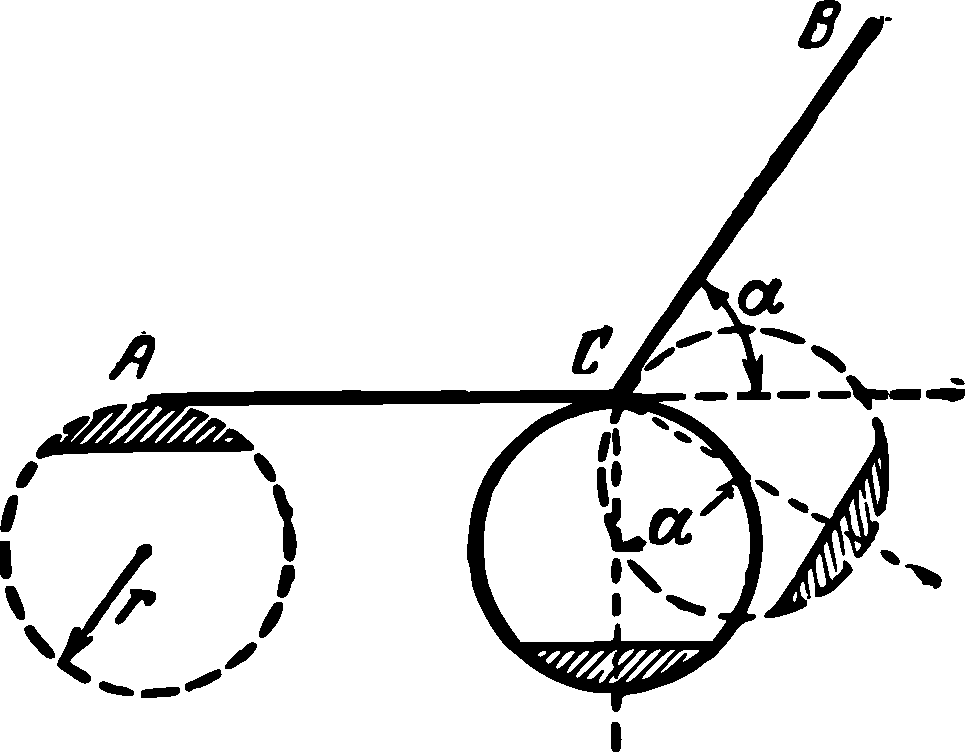
\includegraphics[width=\textwidth]{figures/ch-09/fig-128.pdf}
\sidecaption{How an additional turn appears when the circle is rolling along a polyline.\label{fig-128}}
\end{marginfigure}

Now, after making half a turn, the circle reaches the vertex $ C $, and to assume such a position where it will touch the line $ CB $ at point $ C $, it will rotate together with its centre by an angle equal to $ \alpha $ (these angles are equal, as they have mutually perpendicular sides).

During this rotation, the circle rolls without moving along the segment. This creates the additional part of the full revolution compared to rolling along the straight line.

The additional rotation constitutes such a fraction of the full revolution as the angle $ \alpha $ constitutes of the angle $ 2\pi $, i.e., $ \alpha/2\pi $. Along the segment $ CB $, the circle also makes half a turn, so in total, when moving along the broken line $ ACB $, it will complete $ 1 + \alpha/2\pi $ revolutions.

\begin{marginfigure}[-1cm]%[h!]
\centering
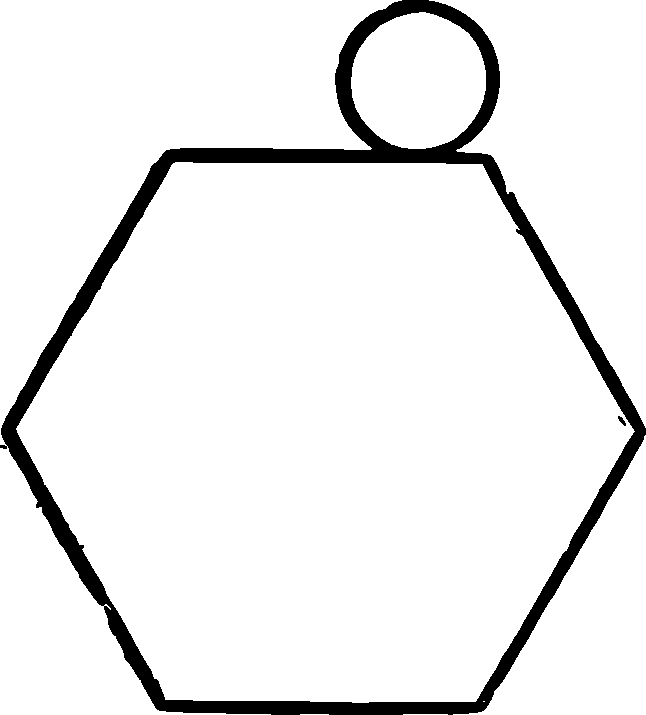
\includegraphics[width=\textwidth]{figures/ch-09/fig-129.pdf}
\sidecaption{How an additional turn appears when the circle is rolling along a poly line.\label{fig-129}}
\end{marginfigure}

Now it's not difficult to imagine how many revolutions a circle rolling on the outside along the sides of a convex regular hexagon (see \figr{fig-129}) should make. It is obvious that it will make as many revolutions as it would wrap around on a straight path equal to the perimeter (i.e., the sum of the sides) of the hexagon, plus the number of revolutions equal to the sum of the external angles of the hexagon divided by $ 2\pi $. Since the sum of the external angles of any convex polygon is constant and equal to $ 4d $ or $ 2\pi $, then $ 2\pi / 2\pi = 1 $.

Thus, when circling the hexagon, as well as any convex polygon, the circle always makes one more revolution than when moving along a straight path equal to the perimeter of the polygon. With an infinite increase in the number of sides, a regular convex polygon approaches a circle. Therefore, all the considerations expressed remain valid for a circle as well. For example, according to the initially posed problem, if one circle rolls along an arc of \ang{120} of another circle equal to it, then the assertion that the moving circle makes not $\nicefrac{1}{3}$ but $\nicefrac{2}{3}$ of a revolution becomes completely geometrically clear.


\section{The Girl on the Tightrope}
\label{sec-9.11}


When a circle rolls along any line lying in the same plane as it, each point of the circle moves in the plane and has its own trajectory, as they say.

Trace the trajectory of any point on a circle rolling along a straight line or a circle, and you will see various curves.\sidenote[][-1cm]{The reader will find a lot of useful and interesting information, as well as examples related to this issue, in the interesting book by G.N. Berman \emph{Cycloid} (1948).} Some of them are depicted in \figr{fig-130} and \ref{fig-131}.

\begin{figure}[h!]
\centering
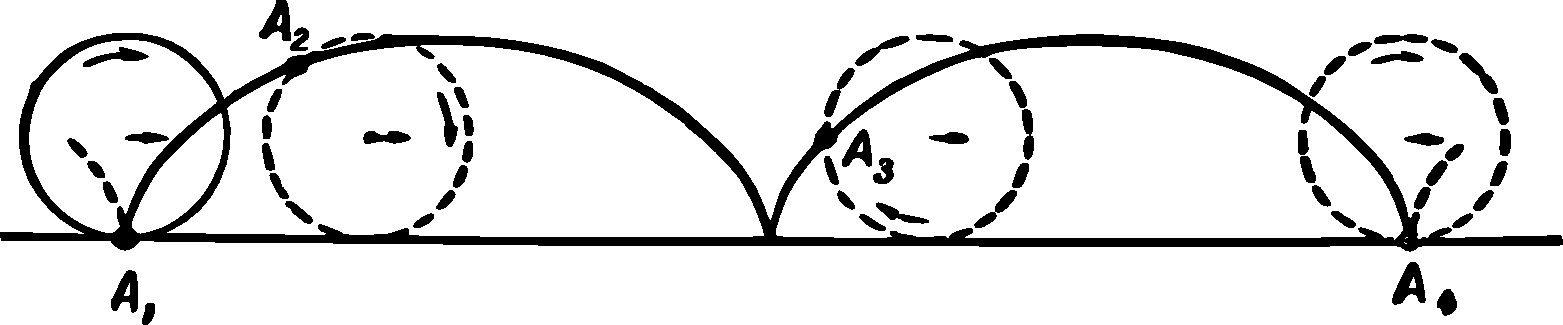
\includegraphics[width=\textwidth]{figures/ch-09/fig-130.pdf}
\sidecaption[][-2cm]{A cycloid is the trajectory of point $A$ of the circumference of a disk rolling in a straight line without sliding.\label{fig-130}}
\end{figure}


The question arises: can a point on a circle rolling along the ``inner side'' of the circumference of another circle (\ref{fig-131}) describe not a curved line, but a straight one? At first glance, it seems impossible. However, I have seen such a construction with my own eyes. It was a toy -- ``the girl on the tightrope'' (\ref{fig-132}). You can easily make it yourself. On a sheet of thick cardboard or plywood, draw a circle with a diameter of 30 cm so that there are margins on the sheet, and extend one of the diameters on both sides.

\begin{marginfigure}[-4cm]%[h!]
\centering
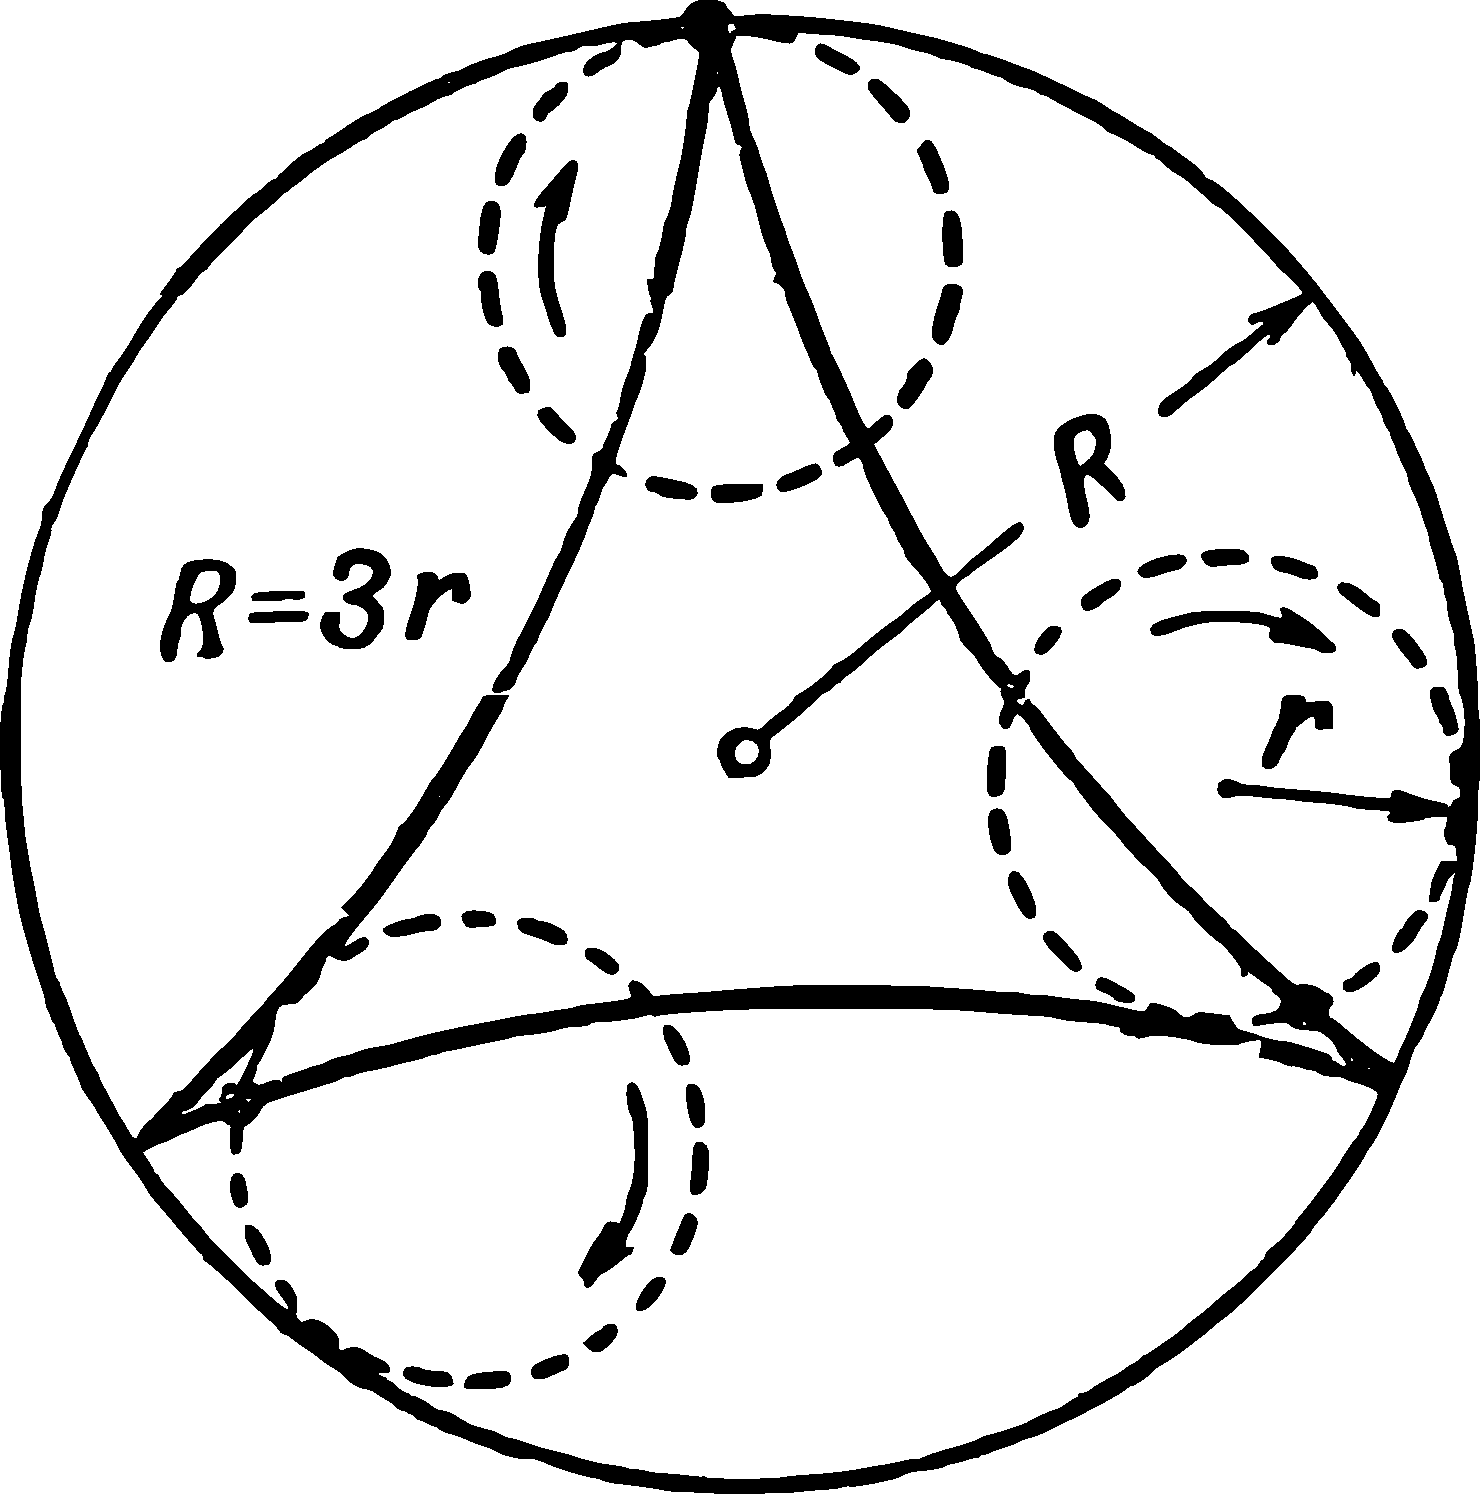
\includegraphics[width=\textwidth]{figures/ch-09/fig-131.pdf}
\sidecaption{Three-point hypocycloid -- the trajectory of points on the circumference of a disk rolling from the inside along the large circumference, where $R = 3r$.\label{fig-131}}
\end{marginfigure}


Insert a needle with a threaded thread into the ends of the diameter, stretch the thread horizontally, and attach both ends to the cardboard (front and back). Cut out the drawn circle, and place another cardboard (or plywood) circle with a diameter of 15 cm in the resulting window. At the very edge of the small circle, insert a needle as shown in \figr{fig-132}, cut out a figure of a girl acrobat from heavy paper, and glue her leg to the head of the needle with sealing wax.

\begin{figure}[h!]
\centering
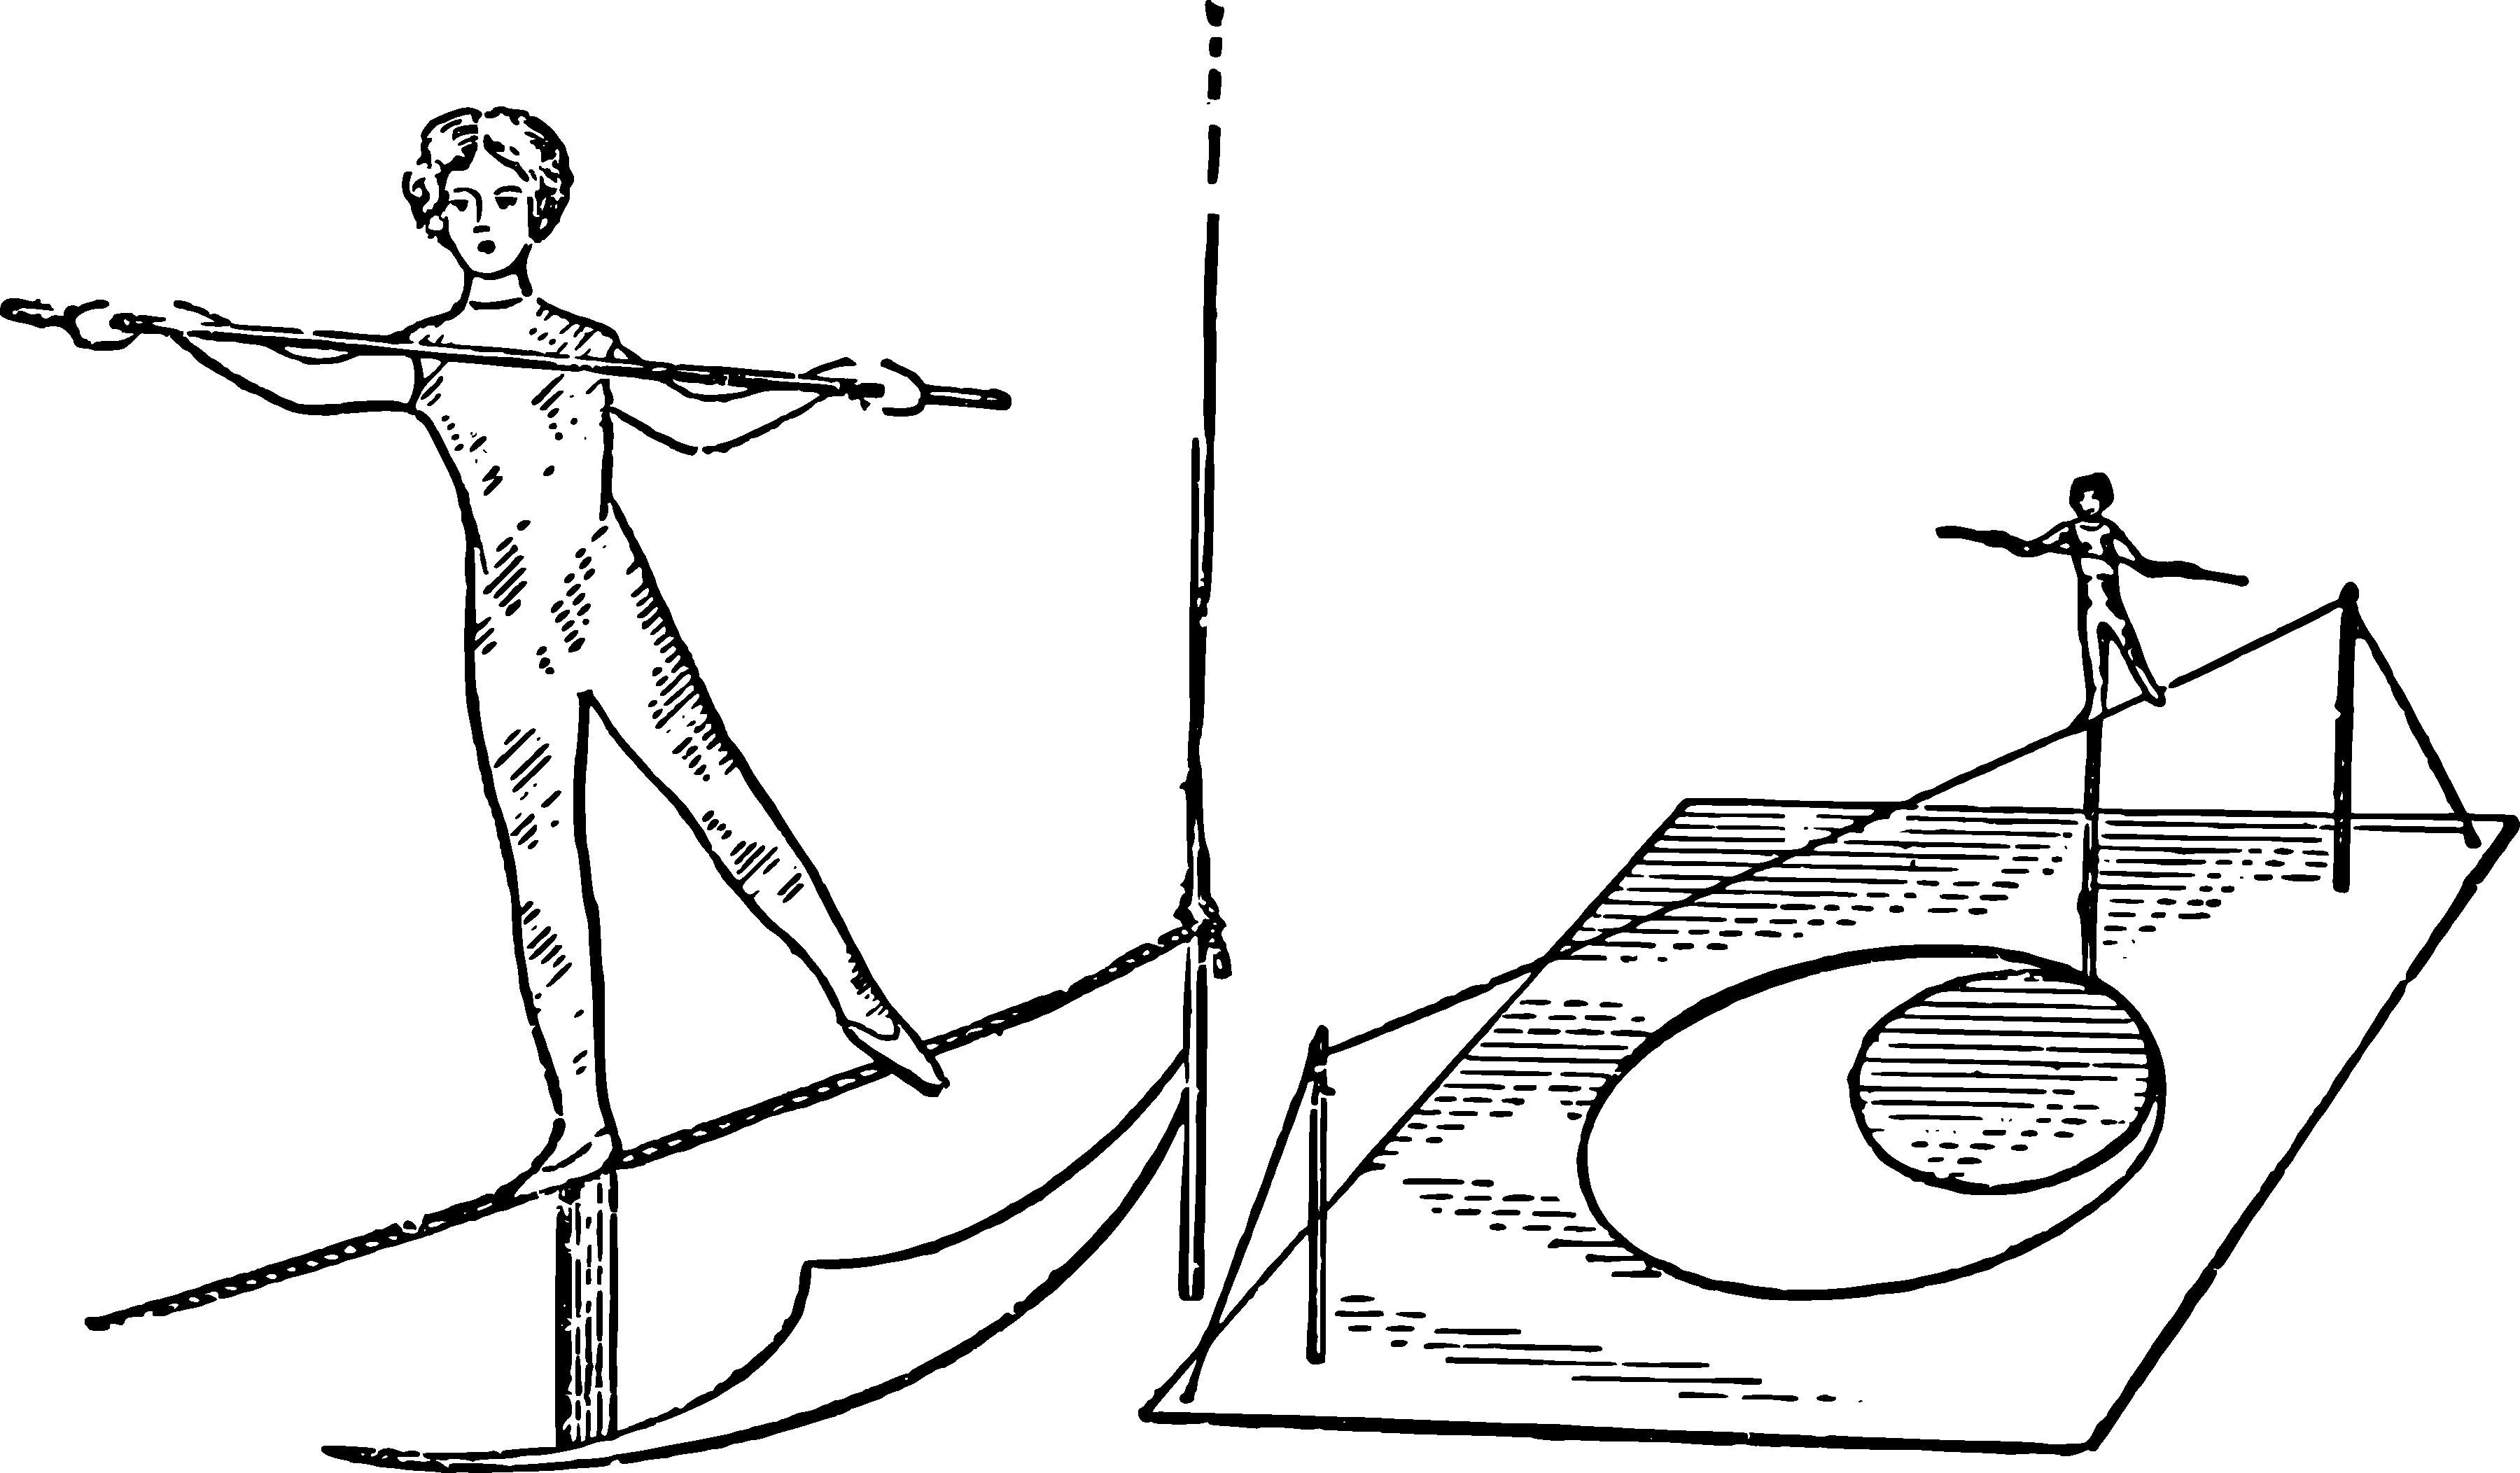
\includegraphics[width=\textwidth]{figures/ch-09/fig-132.pdf}
\sidecaption[][-2cm]{``A girl on a tightrope.'' There are points on a rolling circle that move in a straight line.\label{fig-132}}
\end{figure}

Now try rolling the small circle while pressing it against the edges of the window; the head of the needle, and along with it the figure of the girl, will slide back and forth along the stretched thread. This can only be explained by the fact that the point on the rolling circle to which the needle is attached moves strictly along the diameter of the window.

But why, in a similar case depicted in \figr{fig-131}, does the point on the rolling circle describe not a straight line, but a curved one (it is called a hypocycloid)? It all depends on the ratio of the diameters of the large and small circles. 

\begin{marginfigure}[-2cm]%[h!]
\centering
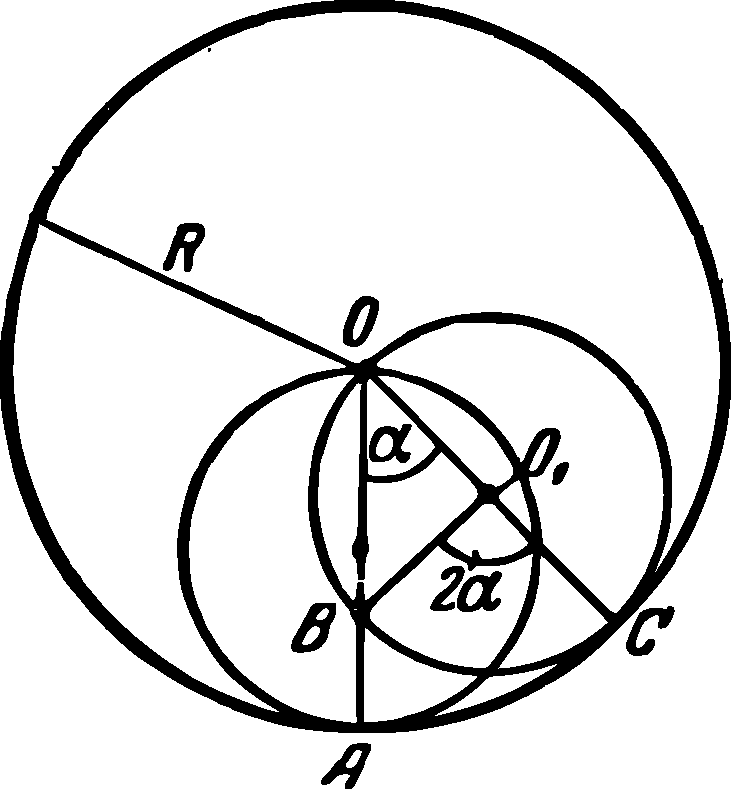
\includegraphics[width=\textwidth]{figures/ch-09/fig-133.pdf}
\sidecaption{Geometric explanation of ``Girl on a tightrope''.\label{fig-133}}
\end{marginfigure}

\ques Prove that if a circle with a diameter half that of a larger circle rolls along the circumference of the larger circle, then during this motion, any point on the circumference of the smaller circle will move along a straight line that is a diameter of the larger circle.



\ans If the diameter of circle $O$ is half the diameter of circle $O_{1}$ (see \figr{fig-133}), then at any moment during the motion of circle $O$, one of its points is at the centre of circle $O_{1}$.

Let's track the movement of point $A$. Suppose the small circle has rolled along arc $AC$. Where will point $A$ be in the new position of circle $O_{1}$?

Obviously, it should be at a point $B$ on its circumference such that arcs $AC$ and $BC$ are equal in length (the circle rolls without slipping). Let $OA = R$ and $\angle AOC = \alpha$. Then $AC = R\alpha$; therefore, $BC = R \alpha$. But since $O_{1}C = R/2$, then $\angle BO_{1}C = R \cdot \alpha/(R/2) = 2 \alpha$, so $\angle BOC$ is half of $2 \alpha/2 = \alpha$, i.e., point $B$ remains on ray $OA$.

The toy described here represents a primitive mechanism for converting rotary motion into linear motion.


\begin{marginfigure}[-2cm]%[h!]
\centering
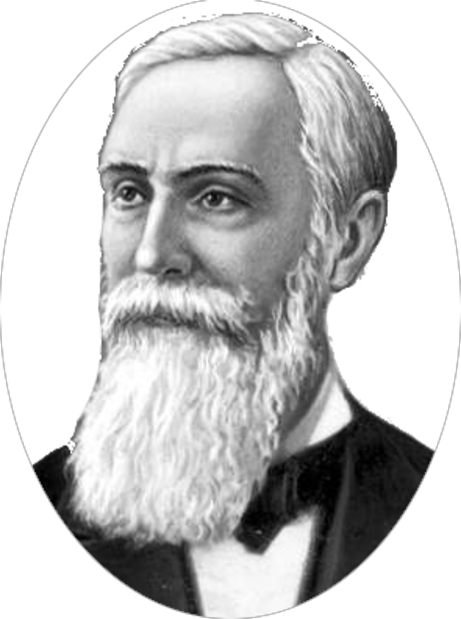
\includegraphics[width=0.8\textwidth]{figures/ch-09/fig-134a.pdf}
\sidecaption{Pafnuty Lvovich Chebyshev (1821–1894).\label{fig-134}}
\end{marginfigure}



The construction of such mechanisms (also called inverters) has interested mechanical engineers since the time of the Ural mechanic Ivan Ivanovich Polzunov, the first inventor of the steam engine. Typically, these mechanisms, which impart linear motion to a point, have a hinge device. 


A significant contribution to the mathematical theory of mechanisms was made by the brilliant Russian mathematician Pafnuty Lvovich Chebyshev (1821–1894) (\figr{fig-134}). He was not only a mathematician but also an outstanding mechanic. He built a model of a ``walking'' machine himself (it is still kept in the USSR Academy of Sciences), a mechanism for a self-propelled chair, and the best counting mechanism of the time -- an arithmetic


\section{The Path Through the Pole}
\label{sec-9.12}


You surely remember the famous flight of the Hero of the Soviet Union M.M. Gromov and his friends from Moscow to San Jacinto via the North Pole, when M.M. Gromov conquered two world records for non-stop flight -- one for a straight-line flight (\SI{10200}{\kilo\meter}) and another for a circuitous route (\SI{11500}{\kilo\meter}) in 62 hours and 17 minutes.

Do you think the plane of the heroes who flew over the pole rotated along with the Earth's axis? This question is often asked, but the correct answer is not always given. Any aircraft, including one flying over the pole, must undoubtedly participate in the rotation of the Earth. This occurs because the flying plane is only separated from the solid part of the Earth but remains connected to the atmosphere and is carried along in the rotational motion around the Earth's axis.

Thus, during the flight over the pole from Moscow to America, the aircraft simultaneously rotated with the Earth around its axis. But what was the path of this flight?

To answer this question correctly, it is necessary to keep in mind that when we say ``a body is in motion,'' it means that the position of the body changes relative to other bodies. The question of the path and movement would not make sense if the frame of reference, or simply put, the body with respect to which the movement occurs, is not specified (or at least implied), as mathematicians say.

Relative to the Earth, M.M. Gromov's aircraft moved almost along Moscow's meridian. Moscow's meridian, like any other, rotates with the Earth around its axis. Therefore, the aircraft adhered to the meridian during the flight and rotated with the Earth. However, this rotation is not reflected in the shape of the flight path for a ground observer because it occurs relative to another body, not the Earth.

Therefore, for those firmly connected to the Earth, the path of this heroic flight through the pole is an arc of a great circle if we assume that the plane moved precisely along the meridian and remained at the same distance from the centre of the Earth.

Now let's pose the question this way: we have the movement of the aircraft relative to the Earth, and we know that the aircraft and the Earth together rotate around the Earth's axis. That is, we have the movement of the aircraft and the Earth relative to some third body. What will be the flight path for an observer connected to this third body?

Let's simplify this unusual problem a bit. Let's imagine the polar region of our planet as a flat disk lying on a plane perpendicular to the Earth's axis. Let this imaginary plane be the ``body'' around which the disk rotates around the Earth's axis, and let a clockwork trolley roll uniformly along one of the diameters of the disk. It represents the plane flying along the meridian through the pole.

What line will be depicted on our plane to represent the path of the trolley (more precisely speaking, any single point of the trolley, for example, its centre of gravity)?

The time it takes for the trolley to travel from one end of the diameter to the other depends on its speed.

We will consider three cases:
\begin{enumerate}
\item The trolley completes its path in 12 hours;
\item It completes the path in 24 hours; and
\item It completes the same path in 48 hours.
\end{enumerate}
The disk completes a full revolution in all cases within 24 hours.



\textbf{The first case (see \figr{fig-135}).} The trolley travels along the diameter of the disk in 12 hours. During this time, the disk completes half a revolution, i.e., it turns by \ang{180}, and points $A$ and $A'$ switch places. In \figr{fig-135}, the diameter is divided into eight equal segments, each of which the trolley covers in 12/8 = 1.5 hours. Let's track where the trolley will be located 1.5 hours after the start of the movement. If the disk were not rotating, the trolley, starting from point $A$, would reach point $b$ after 1.5 hours. But the disk rotates, and in 1.5 hours, it turns by $\ang{180}/8 = \ang{45}$. During this time, point $b$ of the disk moves to point $b'$. An observer standing on the disk and rotating with it would not notice its rotation and would only see that the trolley moved from point $A$ to point $b$. But an observer who is outside the disk and does not participate in its rotation would see something else: for them, the trolley would move along a curved path from point $A$ to point $b'$. Another 1.5 hours later, the observer standing outside the disk would see the trolley at point $c'$. Over the next 1.5 hours, the trolley would move along the arc $c'd'$, and after another 1.5 hours, it would reach the centre $e$.

\begin{marginfigure}[-2cm]%[h!]
\centering
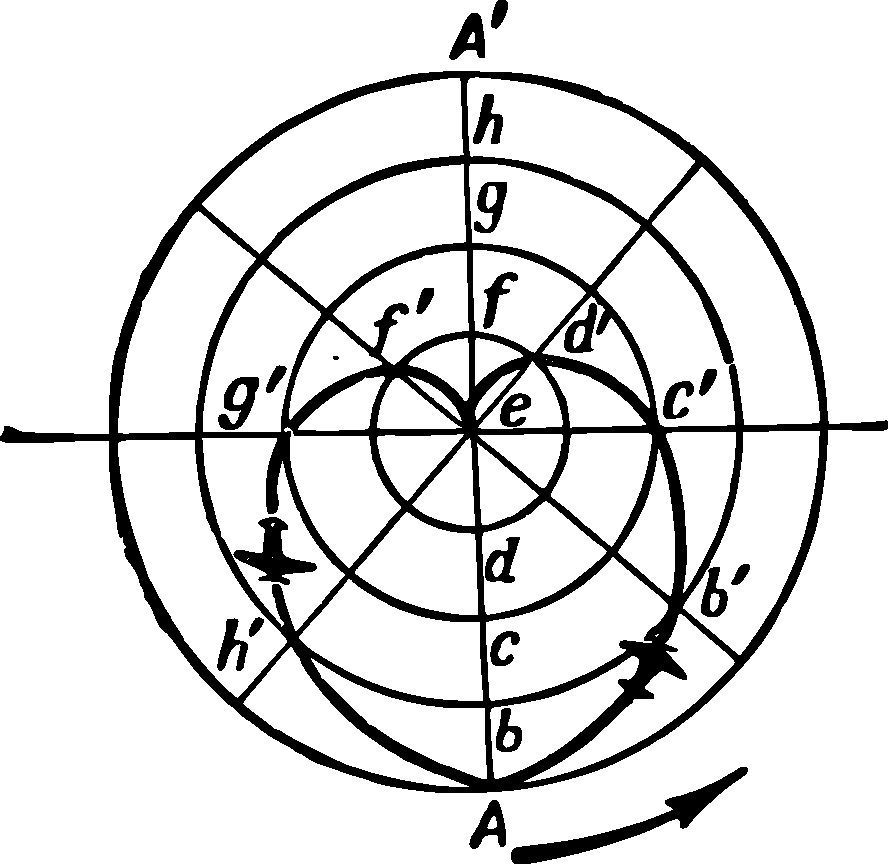
\includegraphics[width=\textwidth]{figures/ch-09/fig-135.pdf}
\sidecaption{Curves that will be described on a fixed plane by a point involved in two movements.\label{fig-135}}
\end{marginfigure}


Continuing to track the movement of the trolley, an observer standing outside the disk would see something completely unexpected: the trolley would describe a curve $ef'g'h'A$ for them, and the movement, strangely enough, would not end at the opposite point of the diameter, but at the starting point.

The solution to this unexpectedness is very simple: during the six hours of the trolley's journey along the second half of the diameter, this radius manages to turn together with the disk by \ang{180} and occupy the position of the first half of the diameter. The trolley rotates together with the disk even at the moment when it passes over its centre. The trolley cannot fit entirely into the centre of the disk; it can only coincide with the centre at one point, and at that moment, it rotates entirely with the disk around this point. The same should happen with the plane when it flies over the pole. So, the journey of the trolley along the diameter of the disk from one end to the other appears differently to different observers. To someone standing on the disk and spinning with it, this path appears as a straight line. But to a stationary observer who is not participating in the rotation of the disk, the movement of the trolley appears as a curve, depicted in \figr{fig-135} and resembling the outline of a heart.

Each of you would see the same curve if, for example, you were observing the flight of the plane from the centre of the Earth relative to an imaginary plane perpendicular to the Earth's axis, under the fantastic condition that the Earth is transparent, and you and the plane are not participating in the Earth's rotation, and if the flight across the pole of the observed plane lasted 12 hours.

Here we have an interesting example of the addition of two motions.

\begin{marginfigure}[-4cm]%[h!]
\centering
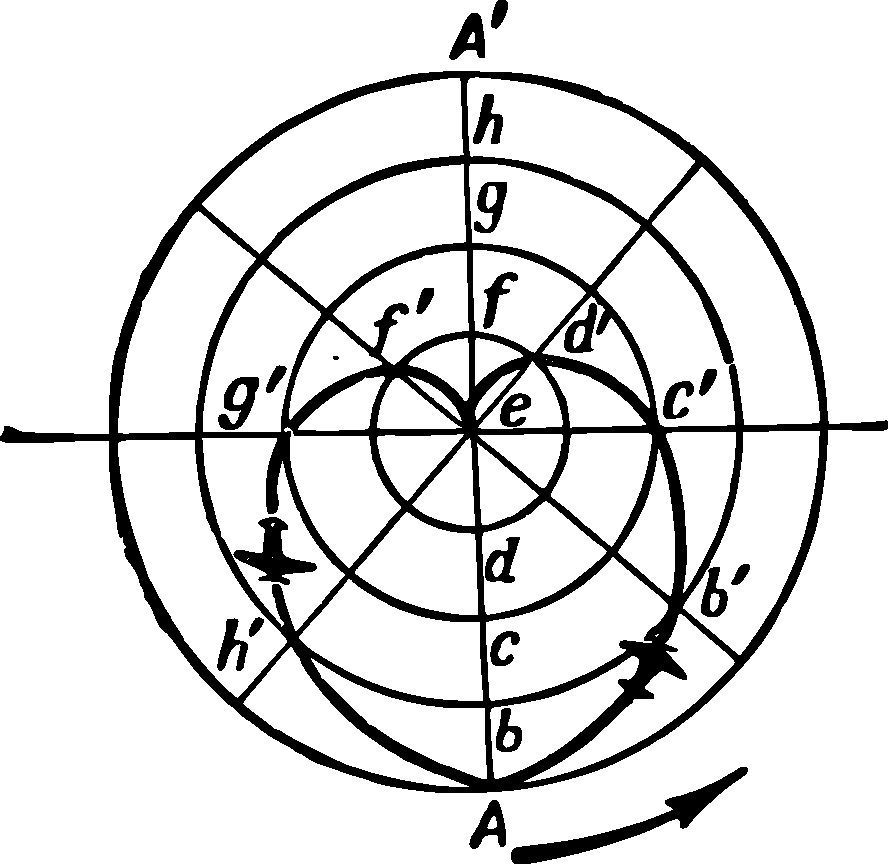
\includegraphics[width=\textwidth]{figures/ch-09/fig-135.pdf}
\sidecaption{Curves that will be described on a fixed plane by a point involved in two movements.\label{fig-136}}
\end{marginfigure}

In fact, the flight across the pole from Moscow to the diametrically opposite point -- the same parallel -- did not last 12 hours, so we will now focus on analysing another preparatory task of the same kind.


\textbf{Second case (\figr{fig-136})}: The trolley traverses the diameter in 24 hours. During this time, the disk completes a full revolution, and then, for an observer stationary relative to the disk, the path of the trolley's movement will take the form of the curve depicted in \figr{fig-136}.

\begin{marginfigure}[-2cm]%[h!]
\centering
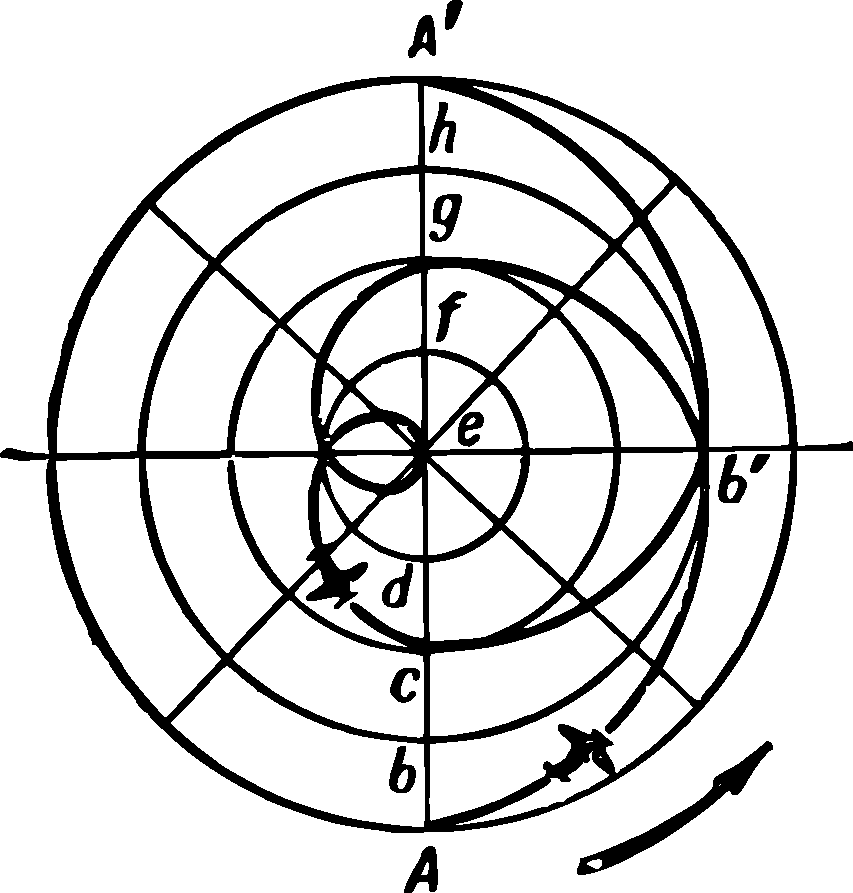
\includegraphics[width=\textwidth]{figures/ch-09/fig-137.pdf}
\sidecaption{Two more curves resulting from the addition of two movements.\label{fig-137}}
\end{marginfigure}



\textbf{Third case (\figr{fig-137})}: The disk still completes a full revolution in 24 hours, but the trolley travels from one end to the other of the diameter in 48 hours.


This time, the trolley covers 1/8 diameters in 48 hours, which equals $48:8 = 6$ hours per diameter. During the same six hours, the disk manages to turn a quarter of a full revolution -- \ang{90}. Therefore, after six hours from the start of the movement, the trolley will move along the diameter (\figr{fig-137}) to point $b$, but the rotation of the disk will shift this point to $b'$. After another six hours, the trolley will reach point $g$, and so on. In 48 hours, the trolley covers the entire diameter, while the disk completes two full revolutions. The result of adding these two movements appears to a stationary observer as an intricate curve, depicted in \figr{fig-137} as a solid line.

The case considered now brings us closer to the true conditions of the flight over the pole. The flight from Moscow to the pole by M. M. Gromov took approximately 24 hours; therefore, an observer at the center of the Earth would see this part of the trajectory as a line almost identical to the first half of the curve shown in \figr{fig-137}. 

\begin{marginfigure}[-1cm]%[h!]
\centering
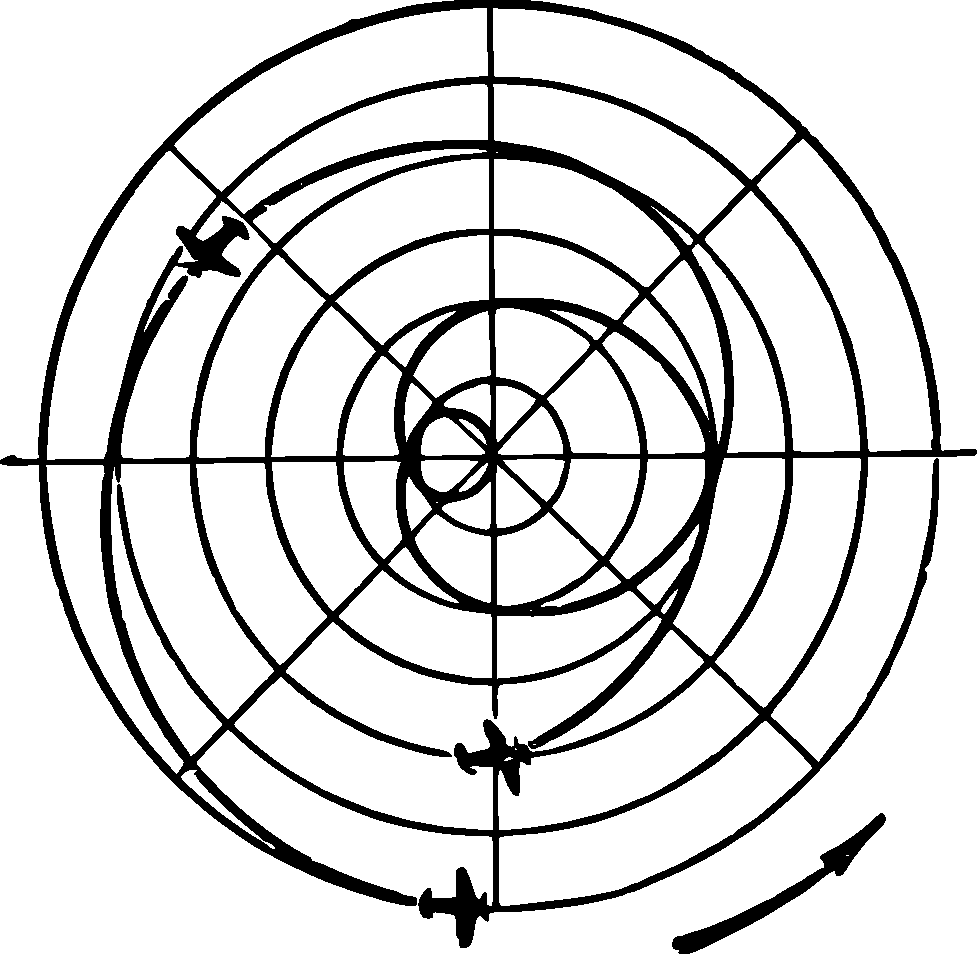
\includegraphics[width=\textwidth]{figures/ch-09/fig-138.pdf}
\sidecaption{The flight path from Moscow to San Jacinto, which would appear to an observer who is not involved in either flight or the rotation of the Earth.\label{fig-138}}
\end{marginfigure}


As for the second part of M. M. Gromov's flight, it lasted approximately one and a half times longer. Additionally, the distance from the pole to San Jacinto is also one and a half times longer than the distance from Moscow to the North Pole. Therefore, the trajectory of the second part of the journey would appear to a stationary observer as a line of the same shape as the first part of the journey but one and a half times longer.




The resulting curve in the end is shown in \figr{fig-138}.

Many might be puzzled by the fact that the starting and ending points of the flight are shown in such close proximity on this diagram.

However, it should not be overlooked that the drawing does not show the simultaneous positions of Moscow and San Jacinto but rather their separation by a time interval of 2.5 hours.

So, this is roughly what the trajectory of M. M. Gromov's flight through the pole would have looked like if it were possible to observe the flight, for example, from the center of the Earth. Can we call this complex twist the true path of the flight over the pole, as opposed to the relative one depicted on maps? No, this motion is also relative: it is referred to some body not participating in the rotation of the Earth around its axis, just as the usual depiction of the flight path is related to the surface of the rotating Earth.

If we could observe the same flight from the Moon or the Sun\sidenote{That is, relative to the coordinate system associated with the Moon or the Sun.}, the flight path would appear to us in yet other ways.

The Moon does not share the Earth's daily rotation, but it orbits our planet once a month. During the 62 hour flight from Moscow to San Jacinto, the Moon would have travelled about \ang{30}, and this could not have gone unnoticed by the trajectory of the flight for a lunar observer. The shape of the air plane's trajectory, considered relative to the Sun, would also be influenced by a third movement -- the rotation of the Earth around the Sun.

``There is no movement of a single body; there is only relative movement,'' says Friedrich Engels in \emph{Dialectics of Nature}.

The task we have just considered convinces us of this in the most vivid way.

\clearpage

\section{For the Drive Belt}
\label{sec-9.13}

When the students of the trade school finished their work, the master ``in farewell'' suggested to those willing to solve such

\ques ``For one of the new installations in our workshop'', said the master, ``we need to sew a drive belt—not just for two pulleys, as is often the case, but immediately for three'', -- and the master showed the students a drive diagram (\figr{fig-139}).

\begin{figure}[h!]
\centering
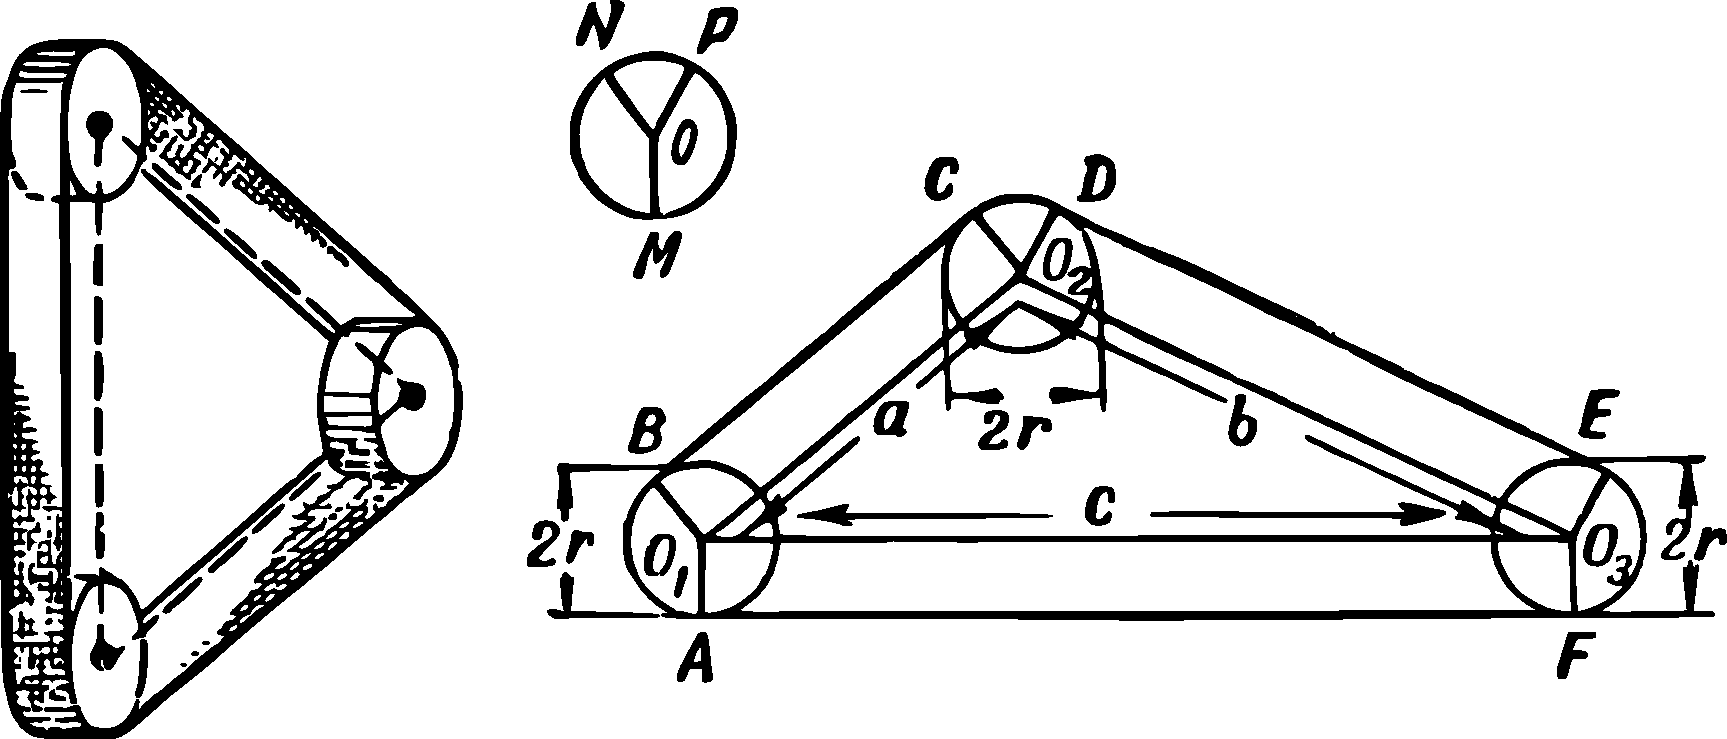
\includegraphics[width=0.9\textwidth]{figures/ch-09/fig-139.pdf}
\sidecaption[][-2cm]{The drive circuit. How to determine the length of the drive belt using only the specified dimensions.\label{fig-139}}
\end{figure}


``All three pulleys,'' he continued, ``have the same dimensions. Their diameter and the distances between their axes are indicated on the diagram.''

``How, knowing these dimensions and without making any additional measurements, can we quickly determine the length of the drive belt?''

The students pondered. Soon, one of them said, ``It seems to me that the only difficulty here is that the sizes of the arcs $AB$, $CD$, and $EF$, around which the belt wraps each pulley, are not indicated on the drawing. To determine the length of each of these arcs, we need to know the magnitude of the corresponding central angle, and it seems to me, we can't do without a protractor.''

``The angles you're talking about'', replied the master, ``can even be calculated using the dimensions indicated on the drawing with the help of trigonometric formulas and tables, but this is a long and complicated path. A protractor is not needed here either, as there is no need to know the length of each arc of interest separately, it is sufficient to know \dots{}''

``Their sum'', some of the boys chimed in, realizing what was at stake.

``Now, go home and bring me your solutions tomorrow.''

Don't rush, reader, to find out what solution the master's students brought him.

After all that has been said by the master, this problem is not difficult to solve independently.


\ans Indeed, the length of the drive belt is determined very simply: to the sum of the distances between the axes of the pulleys, you need to add the length of the circumference of one pulley. If the length of the belt is $ l $, then:
\begin{equation*}%
 l = a + b + c + 2\pi r.
\end{equation*}
Almost all those who attempted the problem guessed that the sum of the lengths of the arcs with which the belt comes into contact equals the entire circumference of one pulley, but not everyone managed to prove it.

From the solutions presented to the master, the following was recognised as the most concise.

Let $BC$, $DE$, and $FA$ be tangents to the circles (see \figr{fig-139}). Draw radii to the points of tangency. Since the circles of the pulleys have equal radii, the figures $O_{1}BCO_{2}$, $ O_{2}DEO_{3} $, and $ O_{1}O_{3}FA $ are rectangles, therefore, $ BC + DE + FA = a + b + c $. It remains to show that the sum of the lengths of the arcs $AB + CD + EF$ equals the total circumference.


To do this, let's construct a circle $O$ with radius $ r $ (see diagram, top). Draw $OM \parallel O_{1}A$, $ON \parallel O_{1}B$, and $OP \parallel O_{2}D$. Then $ \angle MON = \angle AO_{1}B $, $ \angle NOP = \angle CO_{2}D $, and $ \angle ROM = \angle EO_{3}F $ as angles with parallel sides.

Hence, $ AB + CD + EF = MN + NP + PR = 2\pi r $.

Thus, the length of the belt $ l = a + b + c + 2\pi r $.

In the same way, it can be shown that not only for three, but also for any number of equal pulleys, the length of the drive belt will be equal to the sum of the distances between their axes plus the circumference of one pulley.

\begin{figure}[h!]
\centering
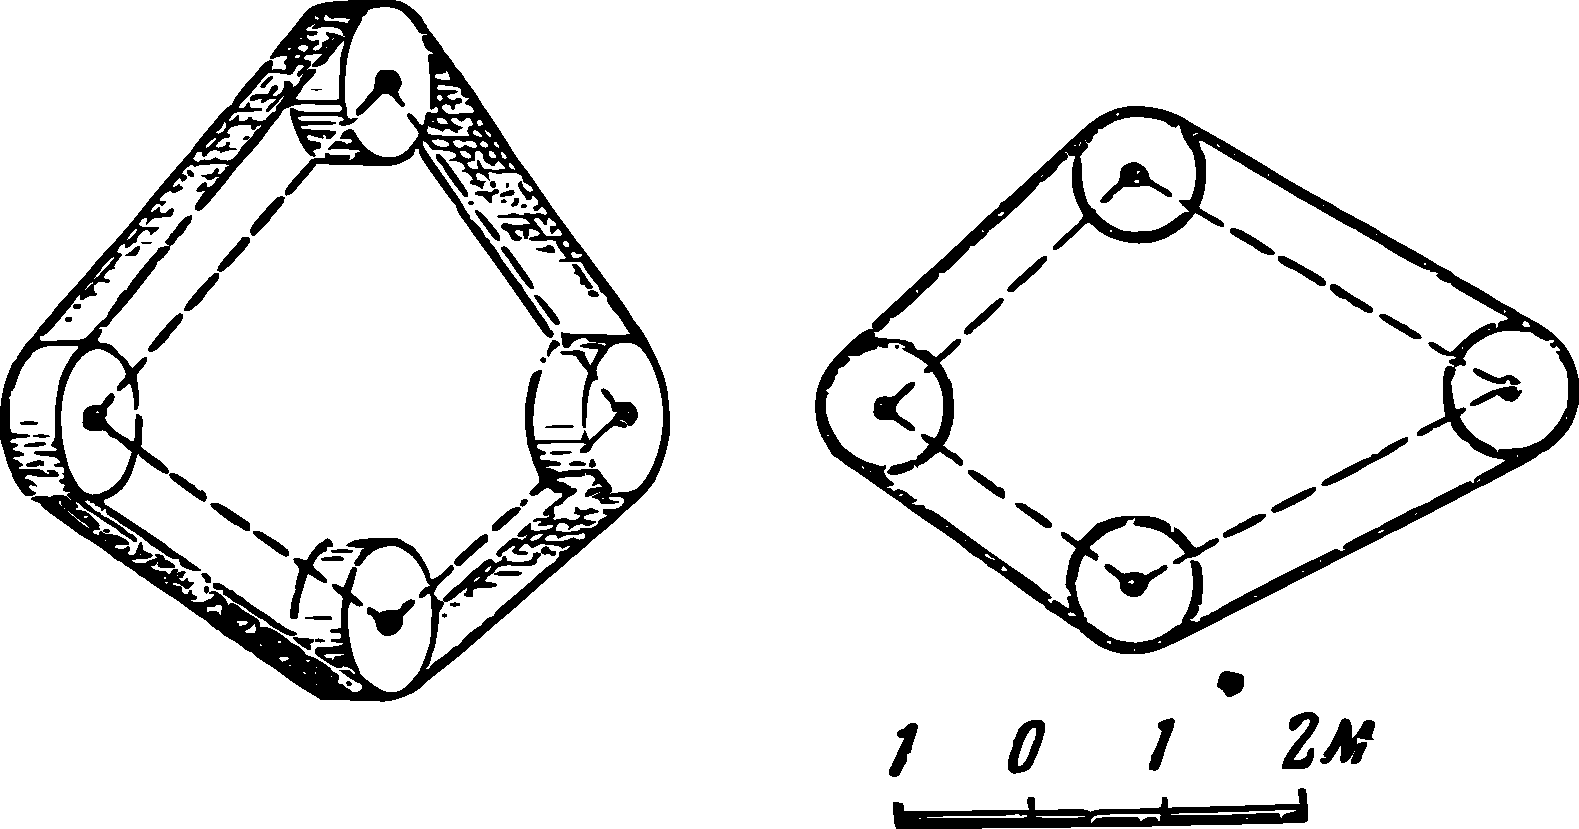
\includegraphics[width=0.9\textwidth]{figures/ch-09/fig-140.pdf}
\sidecaption{Extract the necessary dimensions from the drawing and calculate the length of the conveyor belt.\label{fig-140}}
\end{figure}


\ans On the diagram in \figr{fig-140}, a scheme of a conveyor with four equal rollers is shown (there are intermediate rollers, but they are omitted on the diagram as they do not affect the solution of the problem). Using the scale indicated on the diagram, take the necessary dimensions from the drawing and calculate the length of the conveyor belt.

\clearpage

\section{The Raven's Cleverness}
\label{sec-9.14}

In our school readers in the native language, there is a funny story about a ``clever raven''. This ancient tale tells of a raven suffering from thirst who found a pitcher of water. There was little water in the pitcher, and the raven couldn't reach it with its beak. However, the raven seemed to figure out how to help itself: it started dropping pebbles into the pitcher. As a result of this trickery, the water level rose to the brim of the pitcher, and the raven could quench its thirst.

We won't delve into discussing whether the raven could display such resourcefulness. The case interests us from a geometric perspective. Let's consider the following problem:

\ques Would the raven be able to drink if the water in the pitcher was filled only halfway?



\ans The analysis of the problem will convince us that the method employed by the raven achieves its goal only under certain initial water levels in the pitcher.

For simplicity, let's assume that the pitcher has the shape of a rectangular prism, and the pebbles are spherical and of equal size. It is easy to understand that the water will rise above the level of the pebbles only if the initial water supply occupies a larger volume than all the gaps between the pebbles: then the water will fill the gaps and protrude above the pebbles. Let's try to calculate the volume of these gaps. The easiest calculation is done when the pebbles are arranged in such a way that the centre of each lies on the same vertical line as the centres of the upper and lower pebbles. Let the diameter of a pebble be $d$, and therefore its volume be $\nicefrac{1}{6} \pi d^{3}$, and the volume of the cube circumscribed around it be $d^{3}$. The difference in their volumes, $d^{3} - \nicefrac{1}{6} \pi d^{3}$, is the volume of the unfilled part of the cube, and the ratio 
\begin{equation*}%
\frac{d^{3} - \dfrac{1}{6} \pi d^{3}}{d^{3}} = 0.48
\end{equation*}
means that the unfilled part of each cube constitutes 0.48 of its volume. The sum of the volumes of all the voids relative to the volume of the pitcher is much less than half. The situation hardly changes if the pitcher has a non-prismatic shape and the pebbles are not spherical. In all cases, it can be asserted that if initially the water in the pitcher was poured to below half, the raven would not have been able to raise the water to the brim by dropping pebbles.

If the raven were stronger -- strong enough to pack the pebbles tightly in the pitcher and achieve their dense arrangement -- it would have been able to raise the water more than twice the initial level. But this is beyond its capabilities, and by assuming a loose arrangement of the pebbles, we have not deviated from the real conditions. Moreover, pitchers are usually bulged in the middle; this should also reduce the height of the water rise and corroborate the correctness of our conclusion: if the water stood below half the height of the pitcher, the raven would not have been able to drink.

\begin{center}
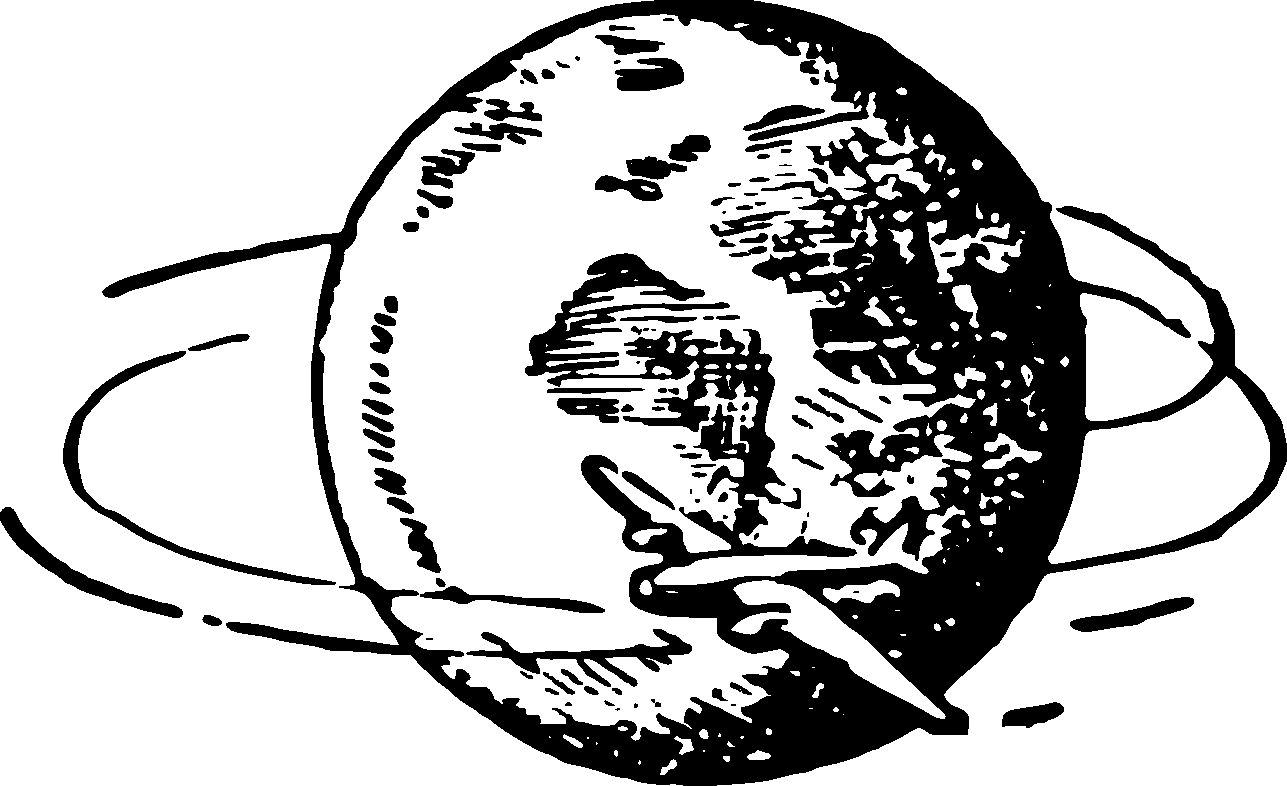
\includegraphics[width=0.3\textwidth]{figures/ch-09/fig-ch-09-tail.pdf}
\end{center}


















